% ICLR 2027 submission -- TempoPB learned allocation policies
%
% Submission reconciliation: numbers.tex is reconstructed from authenticated
% saved results by iclr_manuscript_reconstruct_v2.py. Literal appendix tables
% are checked against the same saved consumer records. See ../REPRODUCE.md.
\documentclass{article}
% Keep independent submission builds byte-stable; this identifier is build
% metadata and does not encode an author, machine, or result.
\pdftrailerid{67D19404F169A5A53D3F714171297F24}
\usepackage{iclr2027_conference,times}
%%%%% NEW MATH DEFINITIONS %%%%%

\usepackage{amsmath,amsfonts,bm}

% Mark sections of captions for referring to divisions of figures
\newcommand{\figleft}{{\em (Left)}}
\newcommand{\figcenter}{{\em (Center)}}
\newcommand{\figright}{{\em (Right)}}
\newcommand{\figtop}{{\em (Top)}}
\newcommand{\figbottom}{{\em (Bottom)}}
\newcommand{\captiona}{{\em (a)}}
\newcommand{\captionb}{{\em (b)}}
\newcommand{\captionc}{{\em (c)}}
\newcommand{\captiond}{{\em (d)}}

% Highlight a newly defined term
\newcommand{\newterm}[1]{{\bf #1}}


% Figure reference, lower-case.
\def\figref#1{figure~\ref{#1}}
% Figure reference, capital. For start of sentence
\def\Figref#1{Figure~\ref{#1}}
\def\twofigref#1#2{figures \ref{#1} and \ref{#2}}
\def\quadfigref#1#2#3#4{figures \ref{#1}, \ref{#2}, \ref{#3} and \ref{#4}}
% Section reference, lower-case.
\def\secref#1{section~\ref{#1}}
% Section reference, capital.
\def\Secref#1{Section~\ref{#1}}
% Reference to two sections.
\def\twosecrefs#1#2{sections \ref{#1} and \ref{#2}}
% Reference to three sections.
\def\secrefs#1#2#3{sections \ref{#1}, \ref{#2} and \ref{#3}}
% Reference to an equation, lower-case.
\def\eqref#1{equation~\ref{#1}}
% Reference to an equation, upper case
\def\Eqref#1{Equation~\ref{#1}}
% A raw reference to an equation---avoid using if possible
\def\plaineqref#1{\ref{#1}}
% Reference to a chapter, lower-case.
\def\chapref#1{chapter~\ref{#1}}
% Reference to an equation, upper case.
\def\Chapref#1{Chapter~\ref{#1}}
% Reference to a range of chapters
\def\rangechapref#1#2{chapters\ref{#1}--\ref{#2}}
% Reference to an algorithm, lower-case.
\def\algref#1{algorithm~\ref{#1}}
% Reference to an algorithm, upper case.
\def\Algref#1{Algorithm~\ref{#1}}
\def\twoalgref#1#2{algorithms \ref{#1} and \ref{#2}}
\def\Twoalgref#1#2{Algorithms \ref{#1} and \ref{#2}}
% Reference to a part, lower case
\def\partref#1{part~\ref{#1}}
% Reference to a part, upper case
\def\Partref#1{Part~\ref{#1}}
\def\twopartref#1#2{parts \ref{#1} and \ref{#2}}

\def\ceil#1{\lceil #1 \rceil}
\def\floor#1{\lfloor #1 \rfloor}
\def\1{\bm{1}}
\newcommand{\train}{\mathcal{D}}
\newcommand{\valid}{\mathcal{D_{\mathrm{valid}}}}
\newcommand{\test}{\mathcal{D_{\mathrm{test}}}}

\def\eps{{\epsilon}}


% Random variables
\def\reta{{\textnormal{$\eta$}}}
\def\ra{{\textnormal{a}}}
\def\rb{{\textnormal{b}}}
\def\rc{{\textnormal{c}}}
\def\rd{{\textnormal{d}}}
\def\re{{\textnormal{e}}}
\def\rf{{\textnormal{f}}}
\def\rg{{\textnormal{g}}}
\def\rh{{\textnormal{h}}}
\def\ri{{\textnormal{i}}}
\def\rj{{\textnormal{j}}}
\def\rk{{\textnormal{k}}}
\def\rl{{\textnormal{l}}}
% rm is already a command, just don't name any random variables m
\def\rn{{\textnormal{n}}}
\def\ro{{\textnormal{o}}}
\def\rp{{\textnormal{p}}}
\def\rq{{\textnormal{q}}}
\def\rr{{\textnormal{r}}}
\def\rs{{\textnormal{s}}}
\def\rt{{\textnormal{t}}}
\def\ru{{\textnormal{u}}}
\def\rv{{\textnormal{v}}}
\def\rw{{\textnormal{w}}}
\def\rx{{\textnormal{x}}}
\def\ry{{\textnormal{y}}}
\def\rz{{\textnormal{z}}}

% Random vectors
\def\rvepsilon{{\mathbf{\epsilon}}}
\def\rvtheta{{\mathbf{\theta}}}
\def\rva{{\mathbf{a}}}
\def\rvb{{\mathbf{b}}}
\def\rvc{{\mathbf{c}}}
\def\rvd{{\mathbf{d}}}
\def\rve{{\mathbf{e}}}
\def\rvf{{\mathbf{f}}}
\def\rvg{{\mathbf{g}}}
\def\rvh{{\mathbf{h}}}
\def\rvu{{\mathbf{i}}}
\def\rvj{{\mathbf{j}}}
\def\rvk{{\mathbf{k}}}
\def\rvl{{\mathbf{l}}}
\def\rvm{{\mathbf{m}}}
\def\rvn{{\mathbf{n}}}
\def\rvo{{\mathbf{o}}}
\def\rvp{{\mathbf{p}}}
\def\rvq{{\mathbf{q}}}
\def\rvr{{\mathbf{r}}}
\def\rvs{{\mathbf{s}}}
\def\rvt{{\mathbf{t}}}
\def\rvu{{\mathbf{u}}}
\def\rvv{{\mathbf{v}}}
\def\rvw{{\mathbf{w}}}
\def\rvx{{\mathbf{x}}}
\def\rvy{{\mathbf{y}}}
\def\rvz{{\mathbf{z}}}

% Elements of random vectors
\def\erva{{\textnormal{a}}}
\def\ervb{{\textnormal{b}}}
\def\ervc{{\textnormal{c}}}
\def\ervd{{\textnormal{d}}}
\def\erve{{\textnormal{e}}}
\def\ervf{{\textnormal{f}}}
\def\ervg{{\textnormal{g}}}
\def\ervh{{\textnormal{h}}}
\def\ervi{{\textnormal{i}}}
\def\ervj{{\textnormal{j}}}
\def\ervk{{\textnormal{k}}}
\def\ervl{{\textnormal{l}}}
\def\ervm{{\textnormal{m}}}
\def\ervn{{\textnormal{n}}}
\def\ervo{{\textnormal{o}}}
\def\ervp{{\textnormal{p}}}
\def\ervq{{\textnormal{q}}}
\def\ervr{{\textnormal{r}}}
\def\ervs{{\textnormal{s}}}
\def\ervt{{\textnormal{t}}}
\def\ervu{{\textnormal{u}}}
\def\ervv{{\textnormal{v}}}
\def\ervw{{\textnormal{w}}}
\def\ervx{{\textnormal{x}}}
\def\ervy{{\textnormal{y}}}
\def\ervz{{\textnormal{z}}}

% Random matrices
\def\rmA{{\mathbf{A}}}
\def\rmB{{\mathbf{B}}}
\def\rmC{{\mathbf{C}}}
\def\rmD{{\mathbf{D}}}
\def\rmE{{\mathbf{E}}}
\def\rmF{{\mathbf{F}}}
\def\rmG{{\mathbf{G}}}
\def\rmH{{\mathbf{H}}}
\def\rmI{{\mathbf{I}}}
\def\rmJ{{\mathbf{J}}}
\def\rmK{{\mathbf{K}}}
\def\rmL{{\mathbf{L}}}
\def\rmM{{\mathbf{M}}}
\def\rmN{{\mathbf{N}}}
\def\rmO{{\mathbf{O}}}
\def\rmP{{\mathbf{P}}}
\def\rmQ{{\mathbf{Q}}}
\def\rmR{{\mathbf{R}}}
\def\rmS{{\mathbf{S}}}
\def\rmT{{\mathbf{T}}}
\def\rmU{{\mathbf{U}}}
\def\rmV{{\mathbf{V}}}
\def\rmW{{\mathbf{W}}}
\def\rmX{{\mathbf{X}}}
\def\rmY{{\mathbf{Y}}}
\def\rmZ{{\mathbf{Z}}}

% Elements of random matrices
\def\ermA{{\textnormal{A}}}
\def\ermB{{\textnormal{B}}}
\def\ermC{{\textnormal{C}}}
\def\ermD{{\textnormal{D}}}
\def\ermE{{\textnormal{E}}}
\def\ermF{{\textnormal{F}}}
\def\ermG{{\textnormal{G}}}
\def\ermH{{\textnormal{H}}}
\def\ermI{{\textnormal{I}}}
\def\ermJ{{\textnormal{J}}}
\def\ermK{{\textnormal{K}}}
\def\ermL{{\textnormal{L}}}
\def\ermM{{\textnormal{M}}}
\def\ermN{{\textnormal{N}}}
\def\ermO{{\textnormal{O}}}
\def\ermP{{\textnormal{P}}}
\def\ermQ{{\textnormal{Q}}}
\def\ermR{{\textnormal{R}}}
\def\ermS{{\textnormal{S}}}
\def\ermT{{\textnormal{T}}}
\def\ermU{{\textnormal{U}}}
\def\ermV{{\textnormal{V}}}
\def\ermW{{\textnormal{W}}}
\def\ermX{{\textnormal{X}}}
\def\ermY{{\textnormal{Y}}}
\def\ermZ{{\textnormal{Z}}}

% Vectors
\def\vzero{{\bm{0}}}
\def\vone{{\bm{1}}}
\def\vmu{{\bm{\mu}}}
\def\vtheta{{\bm{\theta}}}
\def\va{{\bm{a}}}
\def\vb{{\bm{b}}}
\def\vc{{\bm{c}}}
\def\vd{{\bm{d}}}
\def\ve{{\bm{e}}}
\def\vf{{\bm{f}}}
\def\vg{{\bm{g}}}
\def\vh{{\bm{h}}}
\def\vi{{\bm{i}}}
\def\vj{{\bm{j}}}
\def\vk{{\bm{k}}}
\def\vl{{\bm{l}}}
\def\vm{{\bm{m}}}
\def\vn{{\bm{n}}}
\def\vo{{\bm{o}}}
\def\vp{{\bm{p}}}
\def\vq{{\bm{q}}}
\def\vr{{\bm{r}}}
\def\vs{{\bm{s}}}
\def\vt{{\bm{t}}}
\def\vu{{\bm{u}}}
\def\vv{{\bm{v}}}
\def\vw{{\bm{w}}}
\def\vx{{\bm{x}}}
\def\vy{{\bm{y}}}
\def\vz{{\bm{z}}}

% Elements of vectors
\def\evalpha{{\alpha}}
\def\evbeta{{\beta}}
\def\evepsilon{{\epsilon}}
\def\evlambda{{\lambda}}
\def\evomega{{\omega}}
\def\evmu{{\mu}}
\def\evpsi{{\psi}}
\def\evsigma{{\sigma}}
\def\evtheta{{\theta}}
\def\eva{{a}}
\def\evb{{b}}
\def\evc{{c}}
\def\evd{{d}}
\def\eve{{e}}
\def\evf{{f}}
\def\evg{{g}}
\def\evh{{h}}
\def\evi{{i}}
\def\evj{{j}}
\def\evk{{k}}
\def\evl{{l}}
\def\evm{{m}}
\def\evn{{n}}
\def\evo{{o}}
\def\evp{{p}}
\def\evq{{q}}
\def\evr{{r}}
\def\evs{{s}}
\def\evt{{t}}
\def\evu{{u}}
\def\evv{{v}}
\def\evw{{w}}
\def\evx{{x}}
\def\evy{{y}}
\def\evz{{z}}

% Matrix
\def\mA{{\bm{A}}}
\def\mB{{\bm{B}}}
\def\mC{{\bm{C}}}
\def\mD{{\bm{D}}}
\def\mE{{\bm{E}}}
\def\mF{{\bm{F}}}
\def\mG{{\bm{G}}}
\def\mH{{\bm{H}}}
\def\mI{{\bm{I}}}
\def\mJ{{\bm{J}}}
\def\mK{{\bm{K}}}
\def\mL{{\bm{L}}}
\def\mM{{\bm{M}}}
\def\mN{{\bm{N}}}
\def\mO{{\bm{O}}}
\def\mP{{\bm{P}}}
\def\mQ{{\bm{Q}}}
\def\mR{{\bm{R}}}
\def\mS{{\bm{S}}}
\def\mT{{\bm{T}}}
\def\mU{{\bm{U}}}
\def\mV{{\bm{V}}}
\def\mW{{\bm{W}}}
\def\mX{{\bm{X}}}
\def\mY{{\bm{Y}}}
\def\mZ{{\bm{Z}}}
\def\mBeta{{\bm{\beta}}}
\def\mPhi{{\bm{\Phi}}}
\def\mLambda{{\bm{\Lambda}}}
\def\mSigma{{\bm{\Sigma}}}

% Tensor
\DeclareMathAlphabet{\mathsfit}{\encodingdefault}{\sfdefault}{m}{sl}
\SetMathAlphabet{\mathsfit}{bold}{\encodingdefault}{\sfdefault}{bx}{n}
\newcommand{\tens}[1]{\bm{\mathsfit{#1}}}
\def\tA{{\tens{A}}}
\def\tB{{\tens{B}}}
\def\tC{{\tens{C}}}
\def\tD{{\tens{D}}}
\def\tE{{\tens{E}}}
\def\tF{{\tens{F}}}
\def\tG{{\tens{G}}}
\def\tH{{\tens{H}}}
\def\tI{{\tens{I}}}
\def\tJ{{\tens{J}}}
\def\tK{{\tens{K}}}
\def\tL{{\tens{L}}}
\def\tM{{\tens{M}}}
\def\tN{{\tens{N}}}
\def\tO{{\tens{O}}}
\def\tP{{\tens{P}}}
\def\tQ{{\tens{Q}}}
\def\tR{{\tens{R}}}
\def\tS{{\tens{S}}}
\def\tT{{\tens{T}}}
\def\tU{{\tens{U}}}
\def\tV{{\tens{V}}}
\def\tW{{\tens{W}}}
\def\tX{{\tens{X}}}
\def\tY{{\tens{Y}}}
\def\tZ{{\tens{Z}}}


% Graph
\def\gA{{\mathcal{A}}}
\def\gB{{\mathcal{B}}}
\def\gC{{\mathcal{C}}}
\def\gD{{\mathcal{D}}}
\def\gE{{\mathcal{E}}}
\def\gF{{\mathcal{F}}}
\def\gG{{\mathcal{G}}}
\def\gH{{\mathcal{H}}}
\def\gI{{\mathcal{I}}}
\def\gJ{{\mathcal{J}}}
\def\gK{{\mathcal{K}}}
\def\gL{{\mathcal{L}}}
\def\gM{{\mathcal{M}}}
\def\gN{{\mathcal{N}}}
\def\gO{{\mathcal{O}}}
\def\gP{{\mathcal{P}}}
\def\gQ{{\mathcal{Q}}}
\def\gR{{\mathcal{R}}}
\def\gS{{\mathcal{S}}}
\def\gT{{\mathcal{T}}}
\def\gU{{\mathcal{U}}}
\def\gV{{\mathcal{V}}}
\def\gW{{\mathcal{W}}}
\def\gX{{\mathcal{X}}}
\def\gY{{\mathcal{Y}}}
\def\gZ{{\mathcal{Z}}}

% Sets
\def\sA{{\mathbb{A}}}
\def\sB{{\mathbb{B}}}
\def\sC{{\mathbb{C}}}
\def\sD{{\mathbb{D}}}
% Don't use a set called E, because this would be the same as our symbol
% for expectation.
\def\sF{{\mathbb{F}}}
\def\sG{{\mathbb{G}}}
\def\sH{{\mathbb{H}}}
\def\sI{{\mathbb{I}}}
\def\sJ{{\mathbb{J}}}
\def\sK{{\mathbb{K}}}
\def\sL{{\mathbb{L}}}
\def\sM{{\mathbb{M}}}
\def\sN{{\mathbb{N}}}
\def\sO{{\mathbb{O}}}
\def\sP{{\mathbb{P}}}
\def\sQ{{\mathbb{Q}}}
\def\sR{{\mathbb{R}}}
\def\sS{{\mathbb{S}}}
\def\sT{{\mathbb{T}}}
\def\sU{{\mathbb{U}}}
\def\sV{{\mathbb{V}}}
\def\sW{{\mathbb{W}}}
\def\sX{{\mathbb{X}}}
\def\sY{{\mathbb{Y}}}
\def\sZ{{\mathbb{Z}}}

% Entries of a matrix
\def\emLambda{{\Lambda}}
\def\emA{{A}}
\def\emB{{B}}
\def\emC{{C}}
\def\emD{{D}}
\def\emE{{E}}
\def\emF{{F}}
\def\emG{{G}}
\def\emH{{H}}
\def\emI{{I}}
\def\emJ{{J}}
\def\emK{{K}}
\def\emL{{L}}
\def\emM{{M}}
\def\emN{{N}}
\def\emO{{O}}
\def\emP{{P}}
\def\emQ{{Q}}
\def\emR{{R}}
\def\emS{{S}}
\def\emT{{T}}
\def\emU{{U}}
\def\emV{{V}}
\def\emW{{W}}
\def\emX{{X}}
\def\emY{{Y}}
\def\emZ{{Z}}
\def\emSigma{{\Sigma}}

% entries of a tensor
% Same font as tensor, without \bm wrapper
\newcommand{\etens}[1]{\mathsfit{#1}}
\def\etLambda{{\etens{\Lambda}}}
\def\etA{{\etens{A}}}
\def\etB{{\etens{B}}}
\def\etC{{\etens{C}}}
\def\etD{{\etens{D}}}
\def\etE{{\etens{E}}}
\def\etF{{\etens{F}}}
\def\etG{{\etens{G}}}
\def\etH{{\etens{H}}}
\def\etI{{\etens{I}}}
\def\etJ{{\etens{J}}}
\def\etK{{\etens{K}}}
\def\etL{{\etens{L}}}
\def\etM{{\etens{M}}}
\def\etN{{\etens{N}}}
\def\etO{{\etens{O}}}
\def\etP{{\etens{P}}}
\def\etQ{{\etens{Q}}}
\def\etR{{\etens{R}}}
\def\etS{{\etens{S}}}
\def\etT{{\etens{T}}}
\def\etU{{\etens{U}}}
\def\etV{{\etens{V}}}
\def\etW{{\etens{W}}}
\def\etX{{\etens{X}}}
\def\etY{{\etens{Y}}}
\def\etZ{{\etens{Z}}}

% The true underlying data generating distribution
\newcommand{\pdata}{p_{\rm{data}}}
% The empirical distribution defined by the training set
\newcommand{\ptrain}{\hat{p}_{\rm{data}}}
\newcommand{\Ptrain}{\hat{P}_{\rm{data}}}
% The model distribution
\newcommand{\pmodel}{p_{\rm{model}}}
\newcommand{\Pmodel}{P_{\rm{model}}}
\newcommand{\ptildemodel}{\tilde{p}_{\rm{model}}}
% Stochastic autoencoder distributions
\newcommand{\pencode}{p_{\rm{encoder}}}
\newcommand{\pdecode}{p_{\rm{decoder}}}
\newcommand{\precons}{p_{\rm{reconstruct}}}

\newcommand{\laplace}{\mathrm{Laplace}} % Laplace distribution

\newcommand{\E}{\mathbb{E}}
\newcommand{\Ls}{\mathcal{L}}
\newcommand{\R}{\mathbb{R}}
\newcommand{\emp}{\tilde{p}}
\newcommand{\lr}{\alpha}
\newcommand{\reg}{\lambda}
\newcommand{\rect}{\mathrm{rectifier}}
\newcommand{\softmax}{\mathrm{softmax}}
\newcommand{\sigmoid}{\sigma}
\newcommand{\softplus}{\zeta}
\newcommand{\KL}{D_{\mathrm{KL}}}
\newcommand{\Var}{\mathrm{Var}}
\newcommand{\standarderror}{\mathrm{SE}}
\newcommand{\Cov}{\mathrm{Cov}}
% Wolfram Mathworld says $L^2$ is for function spaces and $\ell^2$ is for vectors
% But then they seem to use $L^2$ for vectors throughout the site, and so does
% wikipedia.
\newcommand{\normlzero}{L^0}
\newcommand{\normlone}{L^1}
\newcommand{\normltwo}{L^2}
\newcommand{\normlp}{L^p}
\newcommand{\normmax}{L^\infty}

\newcommand{\parents}{Pa} % See usage in notation.tex. Chosen to match Daphne's book.

\DeclareMathOperator*{\argmax}{arg\,max}
\DeclareMathOperator*{\argmin}{arg\,min}

\DeclareMathOperator{\sign}{sign}
\DeclareMathOperator{\Tr}{Tr}
\let\ab\allowbreak


\usepackage[T1]{fontenc}   % required for \l and \c{e} in Polish district names
\usepackage[utf8]{inputenc}
\usepackage{url}
\usepackage{booktabs}
\usepackage{amsmath}
\usepackage{amssymb}
\usepackage{amsthm}
\usepackage{graphicx}
\usepackage{algorithm}
\usepackage{algpseudocode}
\usepackage{hyperref}
\hypersetup{hidelinks}

% Float placement. Six floats over nine pages exceeds LaTeX's defaults
% (topnumber=2, totalnumber=3), which defers them, wastes vertical space and
% strands tables pages away from the text that discusses them. These are
% placement parameters, not layout changes to the ICLR style.
\setcounter{topnumber}{3}
\setcounter{totalnumber}{4}
\renewcommand{\topfraction}{0.9}
\renewcommand{\textfraction}{0.08}
\renewcommand{\floatpagefraction}{0.75}

\newtheorem{proposition}{Proposition}
\newtheorem{definition}{Definition}

% September 25 submission: authenticated primary-v2 reconstruction.
% Four unavailable corrected-run timings are omitted; the manuscript reports them as not recorded.
\newcommand{\AblApprShareCSD}{0.1699}
\newcommand{\AblApprShareDelta}{-0.0029}
\newcommand{\AblApprShareDeltaAbs}{0.0029}
\newcommand{\AblConcCSD}{0.1633}
\newcommand{\AblConcDelta}{-0.0095}
\newcommand{\AblConcDeltaAbs}{0.0095}
\newcommand{\AblCostShareCSD}{0.1791}
\newcommand{\AblCostShareDelta}{+0.0063}
\newcommand{\AblCostShareDeltaAbs}{0.0063}
\newcommand{\AblDeficitCSD}{0.1760}
\newcommand{\AblDeficitDelta}{+0.0032}
\newcommand{\AblDeficitDeltaAbs}{0.0032}
\newcommand{\AblFullCSD}{0.1728}
\newcommand{\AblFullDelta}{+0.0000}
\newcommand{\AblFullDeltaAbs}{0.0000}
\newcommand{\AblPerCostCSD}{0.1781}
\newcommand{\AblPerCostDelta}{+0.0053}
\newcommand{\AblPerCostDeltaAbs}{0.0053}
\newcommand{\AblationFullCSD}{0.1728}
\newcommand{\AblationWorstDelta}{+0.0063}
\newcommand{\AblationWorstDeltaAbs}{0.0063}
\newcommand{\AblationWorstFeature}{cost\_share}
\newcommand{\ActuatingInert}{20}
\newcommand{\ActuatingLosses}{4}
\newcommand{\ActuatingMeanAll}{-0.0066}
\newcommand{\ActuatingMeanSubset}{-0.0175}
\newcommand{\ActuatingMeanSubsetHi}{-0.0175}
\newcommand{\ActuatingMeanSubsetLo}{-0.0228}
\newcommand{\ActuatingSeries}{12/32}
\newcommand{\ActuatingWins}{8}
\newcommand{\AgeLookupCSD}{0.1624}
\newcommand{\AgeLookupExcl}{0.0452}
\newcommand{\AgeLookupExclVsEndowDiff}{+0.0038}
\newcommand{\AgeLookupExclVsEndowDiffAbs}{0.0038}
\newcommand{\AgeLookupExclVsMESDiff}{+0.0014}
\newcommand{\AgeLookupExclVsMESDiffAbs}{0.0014}
\newcommand{\AgeLookupMultipliers}{0.0564, 0.0528, 0.0895, 20.0855}
\newcommand{\AgeLookupVsSeniorCI}{[-0.0382, -0.0078]}
\newcommand{\AgeLookupVsSeniorDiff}{-0.0217}
\newcommand{\AgeLookupVsSeniorDiffAbs}{0.0217}
\newcommand{\AgeLookupVsSeniorDz}{-0.642}
\newcommand{\AgeLookupVsSeniorP}{= 0.007}
\newcommand{\AgeLookupVsSeniorRecord}{13/0/5}
\newcommand{\AgeLookupVsSeniorWins}{13/18}
\newcommand{\AgeLookupWelfare}{1,261,342}
\newcommand{\AgeLookupWelfareCostPct}{2.5\%}
\newcommand{\AggrReductionPct}{42\%}
\newcommand{\AggrWelfareCostPct}{7\%}
\newcommand{\CompEndowConc}{0.2971}
\newcommand{\CompEndowCost}{0.0422}
\newcommand{\CompEndowFunded}{29.6}
\newcommand{\CompEndowRepTV}{0.0756}
\newcommand{\CompGreedyCostConc}{0.2998}
\newcommand{\CompGreedyCostCost}{0.0390}
\newcommand{\CompGreedyCostFunded}{32.4}
\newcommand{\CompGreedyCostRepTV}{0.0828}
\newcommand{\CompLLMRuleCardConc}{0.2987}
\newcommand{\CompLLMRuleCardCost}{0.0446}
\newcommand{\CompLLMRuleCardFunded}{28.2}
\newcommand{\CompLLMRuleCardRepTV}{0.0748}
\newcommand{\CompLLMRuleCostConc}{0.2930}
\newcommand{\CompLLMRuleCostCost}{0.0669}
\newcommand{\CompLLMRuleCostFunded}{16.2}
\newcommand{\CompLLMRuleCostRepTV}{0.0644}
\newcommand{\CompMESConc}{0.2990}
\newcommand{\CompMESCost}{0.0414}
\newcommand{\CompMESFunded}{30.1}
\newcommand{\CompMESRepTV}{0.0773}
\newcommand{\CompOutcomeCornerConc}{0.2692}
\newcommand{\CompOutcomeCornerCost}{0.1097}
\newcommand{\CompOutcomeCornerFunded}{11.0}
\newcommand{\CompOutcomeCornerRepTV}{0.0664}
\newcommand{\CompOutcomeHeadConc}{0.2953}
\newcommand{\CompOutcomeHeadCost}{0.0393}
\newcommand{\CompOutcomeHeadFunded}{31.6}
\newcommand{\CompOutcomeHeadRepTV}{0.0778}
\newcommand{\ContextualVsAgeLookupCI}{[-0.0105, +0.0301]}
\newcommand{\ContextualVsAgeLookupDiff}{+0.0112}
\newcommand{\ContextualVsAgeLookupDiffAbs}{0.0112}
\newcommand{\ContextualVsAgeLookupDz}{+0.251}
\newcommand{\ContextualVsAgeLookupP}{= 0.311}
\newcommand{\ContextualVsAgeLookupRecord}{5/1/12}
\newcommand{\ContextualVsAgeLookupWins}{5/18}
\newcommand{\CornerExclVsDeployed}{1.8}
\newcommand{\CornerExclVsMES}{3.4}
\newcommand{\CoverageAffectedEditions}{0}
\newcommand{\CoverageMaxUncoveredShare}{0.00\%}
\newcommand{\CoveragePolicyN}{4}
\newcommand{\CoverageScoredEditions}{54}
\newcommand{\CrossCityActiveN}{22}
\newcommand{\CrossCityAllCIHigh}{0.0031}
\newcommand{\CrossCityAllCILow}{-0.0114}
\newcommand{\CrossCityAllDiff}{-0.0039}
\newcommand{\CrossCityAllDiffAbs}{0.0039}
\newcommand{\CrossCityAllLearned}{0.1345}
\newcommand{\CrossCityAllMES}{0.1384}
\newcommand{\CrossCityAllP}{= 0.316}
\newcommand{\CrossCityAllSeriesN}{58}
\newcommand{\CrossCityAllWins}{12/58}
\newcommand{\CrossCityCityN}{2}
\newcommand{\CrossCityElectionN}{273}
\newcommand{\CrossCityGdyniaCIHigh}{0.0000}
\newcommand{\CrossCityGdyniaCILow}{-0.0197}
\newcommand{\CrossCityGdyniaDiff}{-0.0074}
\newcommand{\CrossCityGdyniaDiffAbs}{0.0074}
\newcommand{\CrossCityGdyniaLearned}{0.1301}
\newcommand{\CrossCityGdyniaMES}{0.1375}
\newcommand{\CrossCityGdyniaP}{= 0.500}
\newcommand{\CrossCityGdyniaSeriesN}{22}
\newcommand{\CrossCityGdyniaWins}{2/22}
\newcommand{\CrossCityInertN}{36}
\newcommand{\CrossCityLodzCIHigh}{0.0077}
\newcommand{\CrossCityLodzCILow}{-0.0120}
\newcommand{\CrossCityLodzDiff}{-0.0017}
\newcommand{\CrossCityLodzDiffAbs}{0.0017}
\newcommand{\CrossCityLodzLearned}{0.1373}
\newcommand{\CrossCityLodzMES}{0.1390}
\newcommand{\CrossCityLodzP}{= 0.736}
\newcommand{\CrossCityLodzSeriesN}{36}
\newcommand{\CrossCityLodzWins}{10/36}
\newcommand{\CrossCityMedianProjectsActive}{22.2}
\newcommand{\CrossCityMedianProjectsInert}{6.2}
\newcommand{\CrossCityScoredElectionN}{172}
\newcommand{\CrossCitySeriesN}{58}
\newcommand{\CrossCityStratMaxDiff}{+0.0015}
\newcommand{\CrossCityStratMaxDiffAbs}{0.0015}
\newcommand{\CrossCityStratMaxN}{5}
\newcommand{\CrossCityStratMaxThreshold}{30}
\newcommand{\CrossCityStratMinP}{0.31}
\newcommand{\DegCSD}{0.0000}
\newcommand{\DegEightHundredCSD}{0.0000}
\newcommand{\DegEightHundredExcl}{99.0\%}
\newcommand{\DegEightHundredVoters}{800}
\newcommand{\DegEightyCSD}{0.0000}
\newcommand{\DegEightyExcl}{90.0\%}
\newcommand{\DegEightyVoters}{80}
\newcommand{\DegExcl}{99.0\%}
\newcommand{\DegFourHundredCSD}{0.0000}
\newcommand{\DegFourHundredExcl}{98.0\%}
\newcommand{\DegFourHundredVoters}{400}
\newcommand{\DegGroups}{8}
\newcommand{\DegSupporters}{8}
\newcommand{\DegTwoHundredCSD}{0.0000}
\newcommand{\DegTwoHundredExcl}{96.0\%}
\newcommand{\DegTwoHundredVoters}{200}
\newcommand{\DegVoters}{800}
\newcommand{\DistrictCVCI}{[-0.0396, -0.0205]}
\newcommand{\DistrictCVDiff}{-0.0301}
\newcommand{\DistrictCVDiffAbs}{0.0301}
\newcommand{\DistrictCVExclDiff}{-0.0031}
\newcommand{\DistrictCVExclDiffAbs}{0.0031}
\newcommand{\DistrictCVFoldMeanDiff}{-0.0302}
\newcommand{\DistrictCVFoldMeanDiffAbs}{0.0302}
\newcommand{\DistrictCVFoldWins}{5/5}
\newcommand{\DistrictCVLearnedCSD}{0.1941}
\newcommand{\DistrictCVLearnedExcl}{0.0628}
\newcommand{\DistrictCVMESCSD}{0.2242}
\newcommand{\DistrictCVMESExcl}{0.0660}
\newcommand{\DistrictCVN}{19}
\newcommand{\DistrictCVP}{= 0.0625}
\newcommand{\DistrictCVSeriesP}{< 0.001}
\newcommand{\DistrictCVTies}{0}
\newcommand{\DistrictCVWelfareCostPct}{1.6\%}
\newcommand{\DistrictCVWelfareDeltaPct}{-1.6\%}
\newcommand{\DistrictCVWelfareRatio}{0.984}
\newcommand{\DistrictCVWideCI}{[-0.0477, -0.0235]}
\newcommand{\DistrictCVWideCSDShift}{-0.0054}
\newcommand{\DistrictCVWideDiff}{-0.0355}
\newcommand{\DistrictCVWideDiffAbs}{0.0355}
\newcommand{\DistrictCVWideFoldWins}{5/5}
\newcommand{\DistrictCVWideLearnedCSD}{0.1886}
\newcommand{\DistrictCVWideLearnedExcl}{0.0645}
\newcommand{\DistrictCVWideP}{= 0.0625}
\newcommand{\DistrictCVWideWelfareCostPct}{1.7\%}
\newcommand{\DistrictCVWideWelfareRatio}{0.983}
\newcommand{\DistrictCVWideWins}{17/19}
\newcommand{\DistrictCVWins}{17/19}
\newcommand{\DynamicsStartYear}{2019}
\newcommand{\EndowCSD}{0.1736}
\newcommand{\EndowExcl}{0.0414}
\newcommand{\EndowNumSeeds}{3}
\newcommand{\EndowReductionPct}{13\%}
% UNAVAILABLE corrected-v2 runtime: EndowRuntimeHiMin
% UNAVAILABLE corrected-v2 runtime: EndowRuntimeLoMin
\newcommand{\EndowSeedHi}{0.1738}
\newcommand{\EndowSeedLo}{0.1729}
\newcommand{\EndowSeedSpread}{0.0009}
\newcommand{\EndowSigLLMRuleCardCI}{[-0.0452, -0.0120]}
\newcommand{\EndowSigLLMRuleCardDiff}{-0.0271}
\newcommand{\EndowSigLLMRuleCardDiffAbs}{0.0271}
\newcommand{\EndowSigLLMRuleCardP}{= 0.002}
\newcommand{\EndowSigLLMRuleCardWins}{15/18}
\newcommand{\EndowSigLLMRuleCostCI}{[-0.0629, -0.0209]}
\newcommand{\EndowSigLLMRuleCostDiff}{-0.0406}
\newcommand{\EndowSigLLMRuleCostDiffAbs}{0.0406}
\newcommand{\EndowSigLLMRuleCostP}{< 0.001}
\newcommand{\EndowSigLLMRuleCostWins}{15/18}
\newcommand{\EndowSigMESCI}{[-0.0453, -0.0081]}
\newcommand{\EndowSigMESDiff}{-0.0255}
\newcommand{\EndowSigMESDiffAbs}{0.0255}
\newcommand{\EndowSigMESHolmP}{= 0.023}
\newcommand{\EndowSigMESP}{= 0.012}
\newcommand{\EndowSigMESWins}{11/18}
\newcommand{\EndowSigRESCI}{[-0.0403, -0.0073]}
\newcommand{\EndowSigRESDiff}{-0.0215}
\newcommand{\EndowSigRESDiffAbs}{0.0215}
\newcommand{\EndowSigRESP}{= 0.006}
\newcommand{\EndowSigRESWins}{11/18}
\newcommand{\EndowSigTwoArmCI}{[-0.0232, +0.0208]}
\newcommand{\EndowSigTwoArmDiff}{0.0008}
\newcommand{\EndowSigTwoArmDiffAbs}{0.0008}
\newcommand{\EndowSigTwoArmP}{= 0.949}
\newcommand{\EndowSigTwoArmWins}{7/18}
\newcommand{\EndowVsMES}{-0.0255}
\newcommand{\EndowWelfare}{1,273,257}
\newcommand{\EndowWelfareCostPct}{1.6\%}
\newcommand{\EndowWelfareRatio}{0.984}
\newcommand{\EvalCityList}{Warszawa}
\newcommand{\EvalCityN}{1}
\newcommand{\EvalSeriesN}{18}
\newcommand{\ExternalAlwaysTies}{13}
\newcommand{\ExternalAlwaysWins}{4}
\newcommand{\ExternalCoverageMin}{99.12\%}
\newcommand{\ExternalDecision}{falsified}
\newcommand{\ExternalElectionN}{228}
\newcommand{\ExternalEndowmentActuated}{12}
\newcommand{\ExternalGateFailN}{4}
\newcommand{\ExternalGatePassN}{4}
\newcommand{\ExternalKatowicePrimaryCIHigh}{0.0000}
\newcommand{\ExternalKatowicePrimaryCILow}{-0.0282}
\newcommand{\ExternalKatowicePrimaryDiff}{-0.0117}
\newcommand{\ExternalKatowicePrimaryDiffAbs}{0.0117}
\newcommand{\ExternalKatowicePrimaryExclDelta}{+0.0085}
\newcommand{\ExternalKatowicePrimaryExclDeltaAbs}{0.0085}
\newcommand{\ExternalKatowicePrimaryHolmP}{0.5000}
\newcommand{\ExternalKatowicePrimaryWelfareRatio}{0.9924}
\newcommand{\ExternalKatowiceSeedFortyTwoDiff}{-0.0117}
\newcommand{\ExternalKatowiceSeedFortyTwoDiffAbs}{0.0117}
\newcommand{\ExternalKatowiceSeedFortyTwoExclDelta}{+0.0085}
\newcommand{\ExternalKatowiceSeedFortyTwoExclDeltaAbs}{0.0085}
\newcommand{\ExternalKatowiceSeedFortyTwoWelfareRatio}{0.9924}
\newcommand{\ExternalKatowiceSeedOneDiff}{-0.0125}
\newcommand{\ExternalKatowiceSeedOneDiffAbs}{0.0125}
\newcommand{\ExternalKatowiceSeedOneExclDelta}{+0.0078}
\newcommand{\ExternalKatowiceSeedOneExclDeltaAbs}{0.0078}
\newcommand{\ExternalKatowiceSeedOneWelfareRatio}{0.9913}
\newcommand{\ExternalKatowiceSeedTwoDiff}{-0.0027}
\newcommand{\ExternalKatowiceSeedTwoDiffAbs}{0.0027}
\newcommand{\ExternalKatowiceSeedTwoExclDelta}{+0.0010}
\newcommand{\ExternalKatowiceSeedTwoExclDeltaAbs}{0.0010}
\newcommand{\ExternalKatowiceSeedTwoWelfareRatio}{1.0002}
\newcommand{\ExternalKrakowPrimaryCIHigh}{0.0166}
\newcommand{\ExternalKrakowPrimaryCILow}{-0.0259}
\newcommand{\ExternalKrakowPrimaryDiff}{-0.0026}
\newcommand{\ExternalKrakowPrimaryDiffAbs}{0.0026}
\newcommand{\ExternalKrakowPrimaryExclDelta}{+0.0015}
\newcommand{\ExternalKrakowPrimaryExclDeltaAbs}{0.0015}
\newcommand{\ExternalKrakowPrimaryHolmP}{0.8398}
\newcommand{\ExternalKrakowPrimaryWelfareRatio}{1.0041}
\newcommand{\ExternalKrakowSeedFortyTwoDiff}{-0.0026}
\newcommand{\ExternalKrakowSeedFortyTwoDiffAbs}{0.0026}
\newcommand{\ExternalKrakowSeedFortyTwoExclDelta}{+0.0015}
\newcommand{\ExternalKrakowSeedFortyTwoExclDeltaAbs}{0.0015}
\newcommand{\ExternalKrakowSeedFortyTwoWelfareRatio}{1.0041}
\newcommand{\ExternalKrakowSeedOneDiff}{-0.0138}
\newcommand{\ExternalKrakowSeedOneDiffAbs}{0.0138}
\newcommand{\ExternalKrakowSeedOneExclDelta}{+0.0037}
\newcommand{\ExternalKrakowSeedOneExclDeltaAbs}{0.0037}
\newcommand{\ExternalKrakowSeedOneWelfareRatio}{1.0014}
\newcommand{\ExternalKrakowSeedTwoDiff}{-0.0080}
\newcommand{\ExternalKrakowSeedTwoDiffAbs}{0.0080}
\newcommand{\ExternalKrakowSeedTwoExclDelta}{-0.0014}
\newcommand{\ExternalKrakowSeedTwoExclDeltaAbs}{0.0014}
\newcommand{\ExternalKrakowSeedTwoWelfareRatio}{1.0015}
\newcommand{\ExternalMedianProjects}{18.0}
\newcommand{\ExternalPrimaryLosses}{4}
\newcommand{\ExternalPrimaryTies}{20}
\newcommand{\ExternalPrimaryWins}{8}
\newcommand{\ExternalPriorityActuated}{3}
\newcommand{\ExternalScoreN}{96}
\newcommand{\ExternalScoredElections}{96}
\newcommand{\ExternalSeedFortyTwoMacro}{-0.0072}
\newcommand{\ExternalSeedOneMacro}{-0.0131}
\newcommand{\ExternalSeedSpread}{0.0078}
\newcommand{\ExternalSeedTwoMacro}{-0.0054}
\newcommand{\ExternalSeriesN}{32}
\newcommand{\ExternalSignSwitches}{5}
\newcommand{\ExternalTopThreeShare}{78.90\%}
\newcommand{\FloorClosesExclPct}{59\%}
\newcommand{\FloorClosesWelfarePct}{27\%}
\newcommand{\HandBandHi}{0.1992}
\newcommand{\HandBandLo}{0.1951}
\newcommand{\HandBandWidth}{0.0040}
\newcommand{\HeadReductionPct}{13\%}
\newcommand{\HistoryFreeVsAgeLookupCI}{[-0.0168, +0.0235]}
\newcommand{\HistoryFreeVsAgeLookupDiff}{+0.0069}
\newcommand{\HistoryFreeVsAgeLookupDiffAbs}{0.0069}
\newcommand{\HistoryFreeVsAgeLookupDz}{+0.153}
\newcommand{\HistoryFreeVsAgeLookupP}{= 0.600}
\newcommand{\HistoryFreeVsAgeLookupRecord}{4/1/13}
\newcommand{\HistoryFreeVsAgeLookupWins}{4/18}
\newcommand{\IdentKOneCSD}{0.1058}
\newcommand{\IdentKOneExcl}{0.0858}
\newcommand{\IdentKOneWelfare}{775,230}
\newcommand{\IdentKTwoCSD}{0.1036}
\newcommand{\IdentKTwoExcl}{0.0975}
\newcommand{\IdentKTwoWelfare}{693,752}
\newcommand{\InfeasGreedyCostBudget}{0.05\%}
\newcommand{\InfeasGreedyCostProj}{0.06\%}
\newcommand{\InfeasLearnedEndowBudget}{0.64\%}
\newcommand{\InfeasLearnedEndowProj}{0.31\%}
\newcommand{\InfeasMESBudget}{0.29\%}
\newcommand{\InfeasMESProj}{0.18\%}
\newcommand{\InfeasOutcomeCornerBudget}{25.06\%}
\newcommand{\InfeasOutcomeCornerProj}{10.29\%}
\newcommand{\InfeasOutcomeHeadBudget}{0.43\%}
\newcommand{\InfeasOutcomeHeadProj}{0.41\%}
\newcommand{\InfeasRESBudget}{0.56\%}
\newcommand{\InfeasRESProj}{0.25\%}
\newcommand{\KappaEndowMax}{13.63}
\newcommand{\KappaEndowMean}{7.40}
\newcommand{\KernelDirectCSD}{0.1228}
\newcommand{\KernelDirectExcl}{0.1470}
\newcommand{\KernelDirectUtil}{99.7\%}
\newcommand{\KernelDirectWelfare}{586,114}
\newcommand{\KernelDirectWelfareFactor}{1.00}
\newcommand{\KernelPaymentCompleteCSD}{0.1282}
\newcommand{\KernelPaymentCompleteCSDCI}{[-0.0227, +0.0341]}
\newcommand{\KernelPaymentCompleteCSDDiff}{0.0054}
\newcommand{\KernelPaymentCompleteCSDDiffAbs}{0.0054}
\newcommand{\KernelPaymentCompleteCSDP}{= 0.721}
\newcommand{\KernelPaymentCompleteExcl}{0.0427}
\newcommand{\KernelPaymentCompleteExclCI}{[-0.1313, -0.0773]}
\newcommand{\KernelPaymentCompleteExclDiff}{-0.1043}
\newcommand{\KernelPaymentCompleteExclDiffAbs}{0.1043}
\newcommand{\KernelPaymentCompleteExclP}{< 0.001}
\newcommand{\KernelPaymentCompleteExclReductionPct}{70.9\%}
\newcommand{\KernelPaymentCompleteExclWins}{17/18}
\newcommand{\KernelPaymentCompleteUtil}{98.7\%}
\newcommand{\KernelPaymentCompleteWelfare}{1,168,671}
\newcommand{\KernelPaymentCompleteWelfareFactor}{1.99}
\newcommand{\KernelPaymentOnlyCSD}{0.1140}
\newcommand{\KernelPaymentOnlyExcl}{0.0530}
\newcommand{\KernelPaymentOnlyUtil}{83.6\%}
\newcommand{\KernelPaymentOnlyWelfare}{1,021,566}
\newcommand{\KernelPaymentOnlyWelfareFactor}{1.74}
\newcommand{\KernelStaticFloorCSD}{0.1165}
\newcommand{\KernelStaticFloorExcl}{0.0935}
\newcommand{\KernelStaticFloorUtil}{99.4\%}
\newcommand{\KernelStaticFloorWelfare}{719,168}
\newcommand{\KernelStaticFloorWelfareFactor}{1.23}
\newcommand{\LLMRuleCardCSD}{0.2007}
\newcommand{\LLMRuleCardCostWelfare}{263,710,950,650}
\newcommand{\LLMRuleCardExcl}{0.0466}
\newcommand{\LLMRuleCardWelfare}{1,291,397}
\newcommand{\LLMRuleCostCSD}{0.2142}
\newcommand{\LLMRuleCostCostWelfare}{303,490,724,672}
\newcommand{\LLMRuleCostExcl}{0.0689}
\newcommand{\LLMRuleCostWelfare}{1,009,756}
\newcommand{\LearnedAggrCSD}{0.1153}
\newcommand{\LearnedAggrExcl}{0.0450}
\newcommand{\LearnedAggrFloor}{0.85}
\newcommand{\LearnedAggrGap}{+0.0312}
\newcommand{\LearnedAggrTrainCSD}{0.0841}
\newcommand{\LearnedAggrWelfare}{1,198,311}
\newcommand{\LearnedCornerCSD}{0.1228}
\newcommand{\LearnedCornerExcl}{0.1470}
\newcommand{\LearnedCornerFloor}{0.00}
\newcommand{\LearnedCornerGap}{+0.0531}
\newcommand{\LearnedCornerTrainCSD}{0.0698}
\newcommand{\LearnedCornerWelfare}{586,114}
\newcommand{\LearnedHeadCSD}{0.1728}
\newcommand{\LearnedHeadExcl}{0.0447}
\newcommand{\LearnedHeadFloor}{1.00}
\newcommand{\LearnedHeadGap}{+0.0057}
\newcommand{\LearnedHeadTrainCSD}{0.1671}
\newcommand{\LearnedHeadWelfare}{1,303,057}
\newcommand{\LossSeriesList}{Ochota, Żoliborz, Wilanów, Białołęka}
\newcommand{\MatchedTargetCIHigh}{0.0298}
\newcommand{\MatchedTargetCILow}{-0.0004}
\newcommand{\MatchedTargetDiff}{+0.0148}
\newcommand{\MatchedTargetDiffAbs}{0.0148}
\newcommand{\MatchedTargetDirectCSD}{0.1728}
\newcommand{\MatchedTargetDirectExcl}{0.0447}
\newcommand{\MatchedTargetEndowCSD}{0.1876}
\newcommand{\MatchedTargetEndowExcl}{0.0433}
\newcommand{\MatchedTargetP}{= 0.080}
\newcommand{\MatchedTargetWins}{5/18}
\newcommand{\MultiAllElectionN}{21}
\newcommand{\MultiAllEndowCSD}{0.1891}
\newcommand{\MultiAllEndowDiff}{-0.0088}
\newcommand{\MultiAllEndowDiffAbs}{0.0088}
\newcommand{\MultiAllEndowExclDelta}{-0.0014}
\newcommand{\MultiAllEndowExclDeltaAbs}{0.0014}
\newcommand{\MultiAllEndowGain}{0.0088}
\newcommand{\MultiAllEndowWelfareCostPct}{0.6\%}
\newcommand{\MultiAllEndowWelfareRatio}{0.994}
\newcommand{\MultiAllMESCSD}{0.1979}
\newcommand{\MultiAllMESDiff}{+0.0000}
\newcommand{\MultiAllMESDiffAbs}{0.0000}
\newcommand{\MultiAllMESExclDelta}{+0.0000}
\newcommand{\MultiAllMESExclDeltaAbs}{0.0000}
\newcommand{\MultiAllMESWelfareRatio}{1.000}
\newcommand{\MultiAllOutcomeCSD}{0.1799}
\newcommand{\MultiAllOutcomeDiff}{-0.0180}
\newcommand{\MultiAllOutcomeDiffAbs}{0.0180}
\newcommand{\MultiAllOutcomeExclDelta}{+0.0101}
\newcommand{\MultiAllOutcomeExclDeltaAbs}{0.0101}
\newcommand{\MultiAllOutcomeGain}{0.0180}
\newcommand{\MultiAllOutcomeWelfareCostPct}{9.0\%}
\newcommand{\MultiAllOutcomeWelfareRatio}{0.910}
\newcommand{\MultiAllSeriesN}{17}
\newcommand{\MultiCityN}{3}
\newcommand{\MultiGdyniaElectionN}{12}
\newcommand{\MultiGdyniaEndowCSD}{0.2024}
\newcommand{\MultiGdyniaEndowDiff}{+0.0000}
\newcommand{\MultiGdyniaEndowDiffAbs}{0.0000}
\newcommand{\MultiGdyniaEndowExclDelta}{+0.0000}
\newcommand{\MultiGdyniaEndowExclDeltaAbs}{0.0000}
\newcommand{\MultiGdyniaEndowGain}{0.0000}
\newcommand{\MultiGdyniaEndowWelfareCostPct}{0.0\%}
\newcommand{\MultiGdyniaEndowWelfareRatio}{1.000}
\newcommand{\MultiGdyniaMESCSD}{0.2024}
\newcommand{\MultiGdyniaMESDiff}{+0.0000}
\newcommand{\MultiGdyniaMESDiffAbs}{0.0000}
\newcommand{\MultiGdyniaMESExclDelta}{+0.0000}
\newcommand{\MultiGdyniaMESExclDeltaAbs}{0.0000}
\newcommand{\MultiGdyniaMESWelfareRatio}{1.000}
\newcommand{\MultiGdyniaOutcomeCSD}{0.1966}
\newcommand{\MultiGdyniaOutcomeDiff}{-0.0059}
\newcommand{\MultiGdyniaOutcomeDiffAbs}{0.0059}
\newcommand{\MultiGdyniaOutcomeExclDelta}{+0.0082}
\newcommand{\MultiGdyniaOutcomeExclDeltaAbs}{0.0082}
\newcommand{\MultiGdyniaOutcomeGain}{0.0059}
\newcommand{\MultiGdyniaOutcomeWelfareCostPct}{2.7\%}
\newcommand{\MultiGdyniaOutcomeWelfareRatio}{0.973}
\newcommand{\MultiGdyniaSeriesN}{10}
\newcommand{\MultiLodzElectionN}{7}
\newcommand{\MultiLodzEndowCSD}{0.1721}
\newcommand{\MultiLodzEndowDiff}{-0.0299}
\newcommand{\MultiLodzEndowDiffAbs}{0.0299}
\newcommand{\MultiLodzEndowExclDelta}{-0.0046}
\newcommand{\MultiLodzEndowExclDeltaAbs}{0.0046}
\newcommand{\MultiLodzEndowGain}{0.0299}
\newcommand{\MultiLodzEndowWelfareCostPct}{0.6\%}
\newcommand{\MultiLodzEndowWelfareRatio}{0.994}
\newcommand{\MultiLodzMESCSD}{0.2019}
\newcommand{\MultiLodzMESDiff}{+0.0000}
\newcommand{\MultiLodzMESDiffAbs}{0.0000}
\newcommand{\MultiLodzMESExclDelta}{+0.0000}
\newcommand{\MultiLodzMESExclDeltaAbs}{0.0000}
\newcommand{\MultiLodzMESWelfareRatio}{1.000}
\newcommand{\MultiLodzOutcomeCSD}{0.1688}
\newcommand{\MultiLodzOutcomeDiff}{-0.0331}
\newcommand{\MultiLodzOutcomeDiffAbs}{0.0331}
\newcommand{\MultiLodzOutcomeExclDelta}{+0.0257}
\newcommand{\MultiLodzOutcomeExclDeltaAbs}{0.0257}
\newcommand{\MultiLodzOutcomeGain}{0.0331}
\newcommand{\MultiLodzOutcomeWelfareCostPct}{9.6\%}
\newcommand{\MultiLodzOutcomeWelfareRatio}{0.904}
\newcommand{\MultiLodzSeriesN}{5}
\newcommand{\MultiLublinElectionN}{2}
\newcommand{\MultiLublinEndowCSD}{0.1648}
\newcommand{\MultiLublinEndowDiff}{+0.0000}
\newcommand{\MultiLublinEndowDiffAbs}{0.0000}
\newcommand{\MultiLublinEndowExclDelta}{+0.0000}
\newcommand{\MultiLublinEndowExclDeltaAbs}{0.0000}
\newcommand{\MultiLublinEndowGain}{0.0000}
\newcommand{\MultiLublinEndowWelfareCostPct}{0.0\%}
\newcommand{\MultiLublinEndowWelfareRatio}{1.000}
\newcommand{\MultiLublinMESCSD}{0.1648}
\newcommand{\MultiLublinMESDiff}{+0.0000}
\newcommand{\MultiLublinMESDiffAbs}{0.0000}
\newcommand{\MultiLublinMESExclDelta}{+0.0000}
\newcommand{\MultiLublinMESExclDeltaAbs}{0.0000}
\newcommand{\MultiLublinMESWelfareRatio}{1.000}
\newcommand{\MultiLublinOutcomeCSD}{0.1243}
\newcommand{\MultiLublinOutcomeDiff}{-0.0406}
\newcommand{\MultiLublinOutcomeDiffAbs}{0.0406}
\newcommand{\MultiLublinOutcomeExclDelta}{-0.0198}
\newcommand{\MultiLublinOutcomeExclDeltaAbs}{0.0198}
\newcommand{\MultiLublinOutcomeGain}{0.0406}
\newcommand{\MultiLublinOutcomeWelfareCostPct}{2.5\%}
\newcommand{\MultiLublinOutcomeWelfareRatio}{0.975}
\newcommand{\MultiLublinSeriesN}{2}
\newcommand{\NumSeeds}{4}
\newcommand{\NumSeriesTotal}{19}
\newcommand{\OptimizerLines}{120}
% UNAVAILABLE corrected-v2 runtime: OutcomeRuntimeHiMin
% UNAVAILABLE corrected-v2 runtime: OutcomeRuntimeLoMin
\newcommand{\PartAgeEndowCSD}{0.0907}
\newcommand{\PartAgeEndowP}{= 0.008}
\newcommand{\PartAgeGroups}{4}
\newcommand{\PartAgeMESCSD}{0.1127}
\newcommand{\PartAgeOutcomeCSD}{0.0815}
\newcommand{\PartAgeOutcomeP}{= 0.009}
\newcommand{\PartAgeRESCSD}{0.1106}
\newcommand{\PartAgeSexEndowCSD}{0.1736}
\newcommand{\PartAgeSexEndowP}{= 0.012}
\newcommand{\PartAgeSexGroups}{8}
\newcommand{\PartAgeSexMESCSD}{0.1992}
\newcommand{\PartAgeSexOutcomeCSD}{0.1728}
\newcommand{\PartAgeSexOutcomeP}{= 0.013}
\newcommand{\PartAgeSexRESCSD}{0.1951}
\newcommand{\PartMaxLearnedP}{0.0130}
\newcommand{\PartSexEndowCSD}{0.0352}
\newcommand{\PartSexEndowP}{< 0.001}
\newcommand{\PartSexGroups}{2}
\newcommand{\PartSexMESCSD}{0.0585}
\newcommand{\PartSexOutcomeCSD}{0.0224}
\newcommand{\PartSexOutcomeP}{< 0.001}
\newcommand{\PartSexRESCSD}{0.0558}
\newcommand{\PerSeriesLosses}{4}
\newcommand{\PerSeriesN}{18}
\newcommand{\PerSeriesWins}{14}
\newcommand{\PrimaryBallotN}{821,572}
\newcommand{\PrimaryElectionN}{132}
\newcommand{\PrimaryProjectN}{8,366}
\newcommand{\PrimaryYearHi}{2025}
\newcommand{\PrimaryYearLo}{2016}
\newcommand{\RangeEndowHi}{0.1876}
\newcommand{\RangeEndowLo}{0.1736}
\newcommand{\RangeEndowWidth}{0.0140}
\newcommand{\RangeOutcomeHi}{0.1869}
\newcommand{\RangeOutcomeLo}{0.1153}
\newcommand{\RangeOutcomeWidth}{0.0717}
\newcommand{\SeedMax}{0.1735}
\newcommand{\SeedMin}{0.1695}
\newcommand{\SeedSpread}{0.0040}
\newcommand{\SigAggrCI}{[-0.1083, -0.0592]}
\newcommand{\SigAggrDiff}{-0.0839}
\newcommand{\SigAggrDiffAbs}{0.0839}
\newcommand{\SigAggrP}{< 0.001}
\newcommand{\SigAggrWins}{17/18}
\newcommand{\SigHeadCI}{[-0.0462, -0.0076]}
\newcommand{\SigHeadDiff}{-0.0264}
\newcommand{\SigHeadDiffAbs}{0.0264}
\newcommand{\SigHeadHolmP}{= 0.023}
\newcommand{\SigHeadP}{= 0.013}
\newcommand{\SigHeadWins}{14/18}
\newcommand{\SigTightCI}{[-0.0367, +0.0032]}
\newcommand{\SigTightDiff}{-0.0163}
\newcommand{\SigTightDiffAbs}{0.0163}
\newcommand{\SigTightP}{= 0.133}
\newcommand{\SigTightWins}{11/18}
\newcommand{\SigTighterCI}{[-0.0295, +0.0054]}
\newcommand{\SigTighterDiff}{-0.0122}
\newcommand{\SigTighterDiffAbs}{0.0122}
\newcommand{\SigTighterP}{= 0.197}
\newcommand{\SigTighterWins}{11/18}
\newcommand{\SplitTestEditions}{54}
\newcommand{\SplitTrainEditions}{75}
\newcommand{\StaticTiltCSD}{0.1693}
\newcommand{\StaticTiltExcl}{0.0415}
\newcommand{\StaticTiltWelfare}{1,277,379}
\newcommand{\TestGreedyCSD}{0.2173}
\newcommand{\TestGreedyCostCSD}{0.1991}
\newcommand{\TestGreedyCostExcl}{0.0448}
\newcommand{\TestGreedyCostWelfare}{1,319,325}
\newcommand{\TestGreedyExcl}{0.0813}
\newcommand{\TestGreedyWelfare}{918,508}
\newcommand{\TestHistoricalCSD}{0.2189}
\newcommand{\TestHistoricalExcl}{0.0830}
\newcommand{\TestHistoricalWelfare}{917,379}
\newcommand{\TestMESCSD}{0.1992}
\newcommand{\TestMESExcl}{0.0438}
\newcommand{\TestMESWelfare}{1,293,610}
\newcommand{\TestRESCSD}{0.1951}
\newcommand{\TestRESExcl}{0.0436}
\newcommand{\TestRESWelfare}{1,286,793}
\newcommand{\TiltAlpha}{2.80}
\newcommand{\TiltCIHigh}{-0.0052}
\newcommand{\TiltCILow}{-0.0241}
\newcommand{\TiltCSD}{0.1841}
\newcommand{\TiltDiff}{-0.0150}
\newcommand{\TiltDiffAbs}{0.0150}
\newcommand{\TiltHolmP}{= 0.022}
\newcommand{\TiltMES}{0.1992}
\newcommand{\TiltP}{= 0.007}
\newcommand{\TiltWins}{14/18}
\newcommand{\TransferEndowCSD}{0.1326}
\newcommand{\TransferEndowWelfare}{447,075}
\newcommand{\TransferGreedyCostCSD}{0.0700}
\newcommand{\TransferGreedyCostWelfare}{464,787}
\newcommand{\TransferHistCSD}{0.1324}
\newcommand{\TransferHistWelfare}{320,936}
\newcommand{\TransferMESCSD}{0.1702}
\newcommand{\TransferMESWelfare}{449,934}
\newcommand{\TransferOutcomeCSD}{0.0620}
\newcommand{\TransferOutcomeWelfare}{405,464}
\newcommand{\WarsawHolmFamilyN}{3}
\newcommand{\WarsawMedianProjects}{47.5}
\newcommand{\WarsawScoredElections}{54}
\newcommand{\WorstCohortMale}{17/18}
\newcommand{\WorstCohortSenior}{14/18}
\newcommand{\WorstCohortSeniorMale}{13/18}


\newcommand{\MES}{\textsc{Mes}}
\newcommand{\RES}{\textsc{Res}}
\newcommand{\csd}{\mathrm{CSD}}
\providecommand{\computehardware}{an 18-GB Apple M3 Pro CPU}
% The anonymous code archive will be supplied with the OpenReview supplementary upload.

\title{Coverage Is Not Fairness: Auditing Learned Controls in Participatory Budgeting}

\author{Anonymous authors\\Paper under double-blind review}

\begin{document}
\maketitle

\begin{abstract}
Spending-based group fairness scores can report a perfect result even when
nearly all voters receive no funded project they approved. We examine
cumulative share deficit (CSD), a group-spending measure, alongside voter
coverage in participatory budgeting. We construct a valid allocation with CSD
\DegCSD{} that excludes \DegExcl{} of voters. Next, we hold score weights and
feature definitions fixed and replay the policy through four allocation rules.
At the unpenalized score, iterative payment reduces exclusion from
\KernelDirectExcl{} to \KernelPaymentOnlyExcl{} and increases welfare to
\KernelPaymentOnlyWelfareFactor$\times$ the direct-score value. Adding
approval-count completion brings exclusion to \KernelPaymentCompleteExcl{}
and welfare to \KernelPaymentCompleteWelfareFactor$\times$. Neither payment
rule produces a statistically detectable CSD improvement. On
\EvalSeriesN{} held-out Warsaw series, learned endowments reduce CSD from
\TestMESCSD{} to \EndowCSD{}, but a post-lock, four-parameter age table fitted
on Warsaw training data has a lower mean (\AgeLookupCSD{}). Two locked
external tests, one of learned priority and one of endowments on
\ExternalSeriesN{} projected-support series in two new cities, do not confirm
transfer (decision: \texttt{\ExternalDecision}). Finally, a post-hoc replay
without refitting finds no detectable series-level difference on
\CrossCityAllSeriesN{} native-approval series and identical allocations on
\CrossCityInertN{}. These results support reporting spending-based fairness
together with voter coverage, and learned interventions together with the
allocation changes they produce.
\end{abstract}

\section{Introduction}

Learning can enter a participatory budgeting (PB) procedure at several points,
even when the fairness objective stays the same. A model can change voter
endowments, reorder affordable projects, or score projects for direct budget
fill. We call the learned object a \emph{control surface}. Where it enters the
procedure determines whether it changes the funded set and which allocations
it can produce.

Under the Method of Equal Shares (\MES), learned endowments and project
priorities retain approver-funded payments during the payment phase.
Direct scoring removes this requirement. Small changes to endowments or
priorities may leave the funded set unchanged. The three classes also learn
different objects from different features, so comparing their fitted outcomes
does not isolate the effect of payment.

We first decompose cumulative share deficit (CSD) and construct an allocation
with zero CSD that excludes almost all voters. Next, we fix the score weights
and feature definitions while changing the allocation rule. Each rule generates
its own allocation history, so this replay measures the rule change together
with the history it induces. We then fit policies on Warsaw elections and test
them outside Warsaw. Learned project priority fails its three-city test.
Endowment estimates on projected support sets in two new cities are favorable
in direction but fail the locked criteria. On \CrossCitySeriesN{}
native-approval series, the fixed Warsaw endowment map shows no detectable
series-level difference from Equal Shares and produces identical allocations
on \CrossCityInertN{}. None of the external studies confirms transfer.

\begin{figure}[tb]
\centering
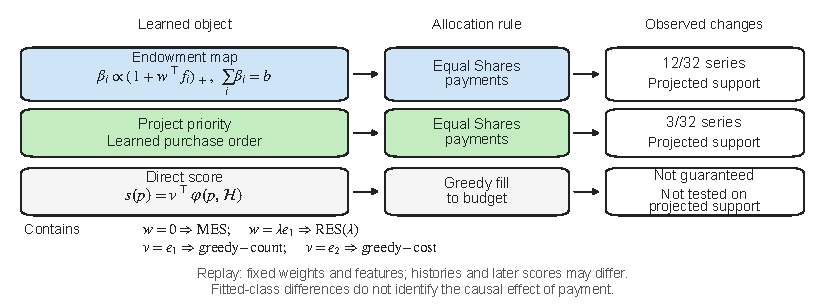
\includegraphics[width=\textwidth]{fig_schematic.pdf}
\caption{Where the three learned interventions enter the allocation process.
Endowment learning changes voter budgets inside Equal Shares. Project-priority
learning changes the order of affordable purchases. Direct scoring fills the
budget without the payment rule. The first two retain Equal Shares payments,
but change allocations on only \ExternalEndowmentActuated{} and
\ExternalPriorityActuated{} of the \ExternalSeriesN{} projected-support series.
Direct scoring was not evaluated on that corpus. Differences between fitted
classes do not identify a causal effect. In the controlled replay, score
weights and feature definitions stay fixed, but later scores can differ
because each rule generates its own deficit history.}
\label{fig:schematic}
\end{figure}

\paragraph{Contributions.}
\begin{itemize}
\item We show that CSD can be zero while exclusion approaches one. The metric
does not measure how many distinct voters are served. In a replay with fixed
score weights and feature definitions, iterative payment reduces exclusion and
raises welfare at the unpenalized score, and approval-count completion adds
coverage. The CSD changes are not statistically detectable. The coverage gains
weaken or reverse at welfare-regularized scores.
\item The fixed endowment map reproduces the unmodified Equal Shares allocation
on most external series. These series have fewer projects on average. That
association does not establish that all endowment changes would leave their
allocations unchanged.
\item The Warsaw results do not establish a benefit from context. A post-lock
static age table reaches lower CSD. Both locked external studies fail, and a
post-hoc native replay without refitting finds no detectable series-level
difference.
\end{itemize}

\section{Problem setting and learned interventions}
\label{sec:setting}

A \emph{repeated participatory budgeting instance} consists of elections
$I_1, \dots, I_T$ and a fixed set of groups $G$. Each election is
\[
I_t \;=\; (P_t,\; c_t,\; b_t,\; N_t,\; A_t)
\]
where $P_t$ contains projects with costs
$c_t : P_t \to \mathbb{R}_{>0}$, $b_t$ is the budget, $N_t$ is the voter set,
and $A_t(i) \subseteq P_t$ is voter $i$'s approval ballot. A voter with recorded
demographics belongs to a group $g(i) \in G$. We write
$N_t^{\mathrm{cov}}\subseteq N_t$ for these voters. Ballots without demographic
coverage still affect the allocation, but not the group ledger. The groups
persist across elections even though the individual voters may change. An
outcome sequence $W_1, \dots, W_T$ satisfies $c_t(W_t) \le b_t$. In this corpus,
$G$ is the set of recorded age-bracket $\times$ sex cells.

\begin{definition}[Attribution and deficit]
\label{def:csd}
In edition $t$, group $g$ receives
$u_t(g) = \sum_{\substack{p \in W_t:\\ n_t^{\mathrm{cov}}(p)>0}}
c_t(p)\, n_{t,g}(p) /
n_t^{\mathrm{cov}}(p)$, where $n_t^{\mathrm{cov}}(p)$ counts covered
approvers of $p$ and $n_{t,g}(p)$ those in $g$; its entitlement is
$e_t(g) = c_t(W_t)\, |g_t| / |N_t^{\mathrm{cov}}|$. The
\emph{cumulative share deficit} after $T$ editions is
\[
\csd_T(g) \;=\; \frac{\sum_{t \le T}\bigl(e_t(g) - u_t(g)\bigr)}
                     {\sum_{t \le T} e_t(g)} .
\]
\end{definition}

We attribute spending only for projects with at least one approver whose
demographics are recorded, but entitlement includes all funded projects. A
funded project with no covered approver would therefore create an artificial
deficit for every group. We found no such project across
\CoverageScoredEditions{} scored elections and \CoveragePolicyN{} policies.
The largest budget share spent on such projects is
\CoverageMaxUncoveredShare{}, so this attribution issue does not affect the
reported comparisons.

Entitlement uses the amount spent rather than the nominal budget. This separates
underspending from unequal distribution. If every funded project has a
covered approver, the unnormalized gaps $e_t(g)-u_t(g)$ sum to zero across
groups. For each series, we accumulate $\csd$ over its scored elections and take
the largest group value. We then average these series-level maxima with equal
weight. A policy carries its own history through $\mathcal{H}_{t-1}$, but the
reported ledger begins with the scored period. Exclusion is also averaged
equally across series, whereas welfare is summed.

CSD measures how spending is distributed; it is not a standard PB axiom. It combines the
share attribution used by Equal Shares
\citep{peters2020welfarism} with a longitudinal equality-of-resources ledger
\citep{maly2023equality}. The ledger compares cumulative group shares but does
not require an allocation to serve many distinct voters.
Proposition~\ref{prop:representative} states this limitation exactly.

We report two additional outcomes. \emph{Welfare} counts (voter, funded project)
approval pairs, or equivalently the number of approved funded projects summed
over voters. The \emph{exclusion rate} is the share of voters who receive none
of their approved projects. Neither enters the objective except through the
soft welfare target in Section~\ref{sec:method}.

\subsection{Three learned intervention classes}
\label{sec:method}

Figure~\ref{fig:schematic} shows where each learned object enters the allocation
process. Appendix~\ref{app:features} gives the feature formulas and optimizer
details.

\paragraph{Learned endowments (payment retained).}
Equal Shares purchases projects at the smallest price $\rho$ for which their
approvers can cover the cost. Approver $i$ pays
$\min(\beta_i, \rho)$ from a personal endowment. Standard \MES{} uses uniform
$\beta_i = b_t/|N_t|$. The learned variant sets
$\beta_i = (b_t/|N_t|)\bigl(1 + w^{\top} f(g(i), \mathcal{H}_{t-1})\bigr)_{+}$,
and rescales the values to sum to $b_t$, falling back to uniform endowments if
all values are zero. A voter without recorded demographics receives the uniform
value before the common rescaling. The six features record
the group's carried deficit per capita, deficit normalized by cumulative
entitlement, size relative to an equal split, mean ballot length, mean cost per
approval, and approval overlap. The last three are expressed as deviations.
Clamping, rescaling, and the fallback ensure nonnegative endowments summing to
the budget. Each reported \MES-family outcome uses the same
approval-count completion (Algorithm~\ref{alg:mes}). Payment-phase winners are
paid for entirely by their approvers. Completion is outside this payment accounting.

\paragraph{Learned project priorities (payment retained).}
This class changes which affordable project is bought next, while retaining
Equal Shares balances and approver-funded payments. Setting every learned
utility to zero reproduces ordinary \MES{} exactly. The learned priority
changes the order of purchases, not the payment rule. In the fresh-city study,
it changes allocations on only \ExternalPriorityActuated{} series.

\paragraph{Learned direct scores (payment discarded).}
We score each project as $s(p) = v^{\top}\phi(p, \mathcal{H}_{t-1})$ and fund
projects in descending score order subject to the budget. Ties are broken by
ascending cost and then project identifier. The five features are approval share, approvals per
unit cost, cost share, a deficit-weighted share of $p$'s covered approvers, and
the concentration of $p$'s support across groups. This class has no
proportionality guarantee. It is a direct-selection comparison, not a
one-factor ablation of the payment rule.

\paragraph{Warsaw fitting and the soft welfare target.}
We fit the endowment and direct-score classes on the training elections with
covariance matrix adaptation evolution strategy (CMA-ES). The initial means are
\RES$(1)$ for endowments and greedy approvals-per-cost for direct scores. These
vectors initialize the search but do not automatically remain among the fitted
candidates. We replay and report every baseline separately. For each class,
target, and seed, one weight vector is optimized jointly across the training
series and frozen before held-out evaluation. The loss is the equal-weighted mean of the
series-level worst-group $\csd$ plus
$\mu \max(0, \tau - \text{welfare}/\text{welfare}_{\MES})$. This penalty
does not impose a hard welfare constraint. It is zero for any
candidate whose welfare ratio meets the target. Once the target exceeds every
attainable welfare ratio, increasing it further adds the same offset to every
candidate, so their ranking no longer changes (Appendix~\ref{app:optim}).

\subsection{Containment of deployed rules}
\label{sec:containment}

Each learned class can reproduce different hand-designed rules. We check the
following identities by running the policies:
\[
w = \mathbf{0} \;\Rightarrow\; \MES, \qquad
w = \lambda e_1 \;\Rightarrow\; \RES(\lambda), \qquad
v = e_1 \;\Rightarrow\; \text{greedy by approval count}.
\]
The first two identities hold with zero numerical error on all
\NumSeriesTotal{} series for
$\lambda \in \{0, 0.25, 0.5, 0.75, 1\}$. The direct class does not contain
\MES{}. Appendix Table~\ref{tab:res-grid} lists every tested \RES{} intensity.
These values concern only the endowment class. In the direct class, $v=e_1$ and
$v=e_2$ recover greedy approval count and greedy approvals per cost, with exact
winner-set equality on all \PrimaryElectionN{} elections. The project-priority
code also reproduces ordinary \MES{} at zero project utility on every
multi-city election in the locked study.

The direct approval-count check found a counting error. The learned score had
counted only ballots with demographic coverage, whereas the deployed rule
counts every ballot. This difference reordered projects in four elections.

\section{Why low CSD can coexist with exclusion}
\label{sec:theory}

We first ask what a low CSD score tells us about voter coverage. We show that
CSD can be zero while almost no voter is served, then derive the support
condition imposed by the Equal Shares payment phase. To examine how the
allocation rule affects coverage, we replay one fixed score function through
different rules. Section~\ref{sec:frontier} compares the fitted classes
separately. Those classes use different objects and features, so their
differences cannot isolate the effect of approver-funded payment.

\begin{proposition}[Representative-support degeneracy]
\label{prop:representative}
Assume every group and every funded project's covered-approver set is nonempty.
Let $s_{t,g}=|g_t|/|N_t^{\mathrm{cov}}|$, let
$q_{t,g}(p)=n_{t,g}(p)/n_t^{\mathrm{cov}}(p)$ be group $g$'s share among
project $p$'s covered approvers, and let
$E_g=\sum_t c_t(W_t)s_{t,g}>0$. Then
\[
\csd_T(g)=1-\sum_t\sum_{p\in W_t}
\underbrace{\frac{c_t(p)s_{t,g}}{E_g}}_{\text{weights sum to }1}
\frac{q_{t,g}(p)}{s_{t,g}}.
\]
If $|q_{t,g}(p)/s_{t,g}-1|\le\epsilon$ for every funded project and group, then
$|\csd_T(g)|\le\epsilon$. Yet for any positive rational group shares and
$\delta>0$, an
instance exists with $\csd(g)=0$ for every group and exclusion at least
$1-\delta$.
\end{proposition}

The construction funds one project that costs the entire budget and whose
approvers match the electorate's group shares. All other voters approve only
an unfunded dummy project. With \DegSupporters{} supporters among
\DegVoters{} voters, the implemented ledger reports CSD \DegCSD{} and
exclusion \DegExcl{}. Spending shares match entitlements exactly, yet almost
everyone receives nothing. This construction demonstrates a limitation of CSD;
it is not an outcome of a fitted policy. Appendix~\ref{app:degeneracy} provides
the proof and executable checks.

The learned endowment policies do not approach this extreme in the Warsaw
data. Their payment phase must satisfy the following support condition.
Greedy completion is not subject to it.

\begin{proposition}[Support floor]
\label{prop:support}
Let $W_{\mathrm{pay}}$ be the projects bought during the Equal Shares payment
phase on instance $(P, c, b, N, A)$ under endowments $\beta \ge 0$ with
$\sum_i \beta_i = b$. Then every $p \in W_{\mathrm{pay}}$
satisfies $\sum_{i \in A(p)} \beta_i \ge c(p)$. Consequently, if
$\beta_i \le \kappa \cdot b / |N|$ for all $i$, then
\[
\frac{|A(p)|}{|N|} \;\ge\; \frac{c(p)}{\kappa\, b}
\qquad\text{for every }p\in W_{\mathrm{pay}} .
\]
\end{proposition}

Appendix~\ref{app:proof} proves the proposition.

During the payment phase, more expensive projects require proportionally more
approvers. Raising the endowment cap weakens this support floor linearly in
$\kappa$. Direct score-and-fill has no corresponding restriction.

The fitted map's per-series cap ratio averages \KappaEndowMean{} and reaches
\KappaEndowMax{}. Its support floor is therefore much weaker than the fixed
$\kappa = 1$ reference in Table~\ref{tab:infeasible}. A large $\kappa$ leaves
little restriction, which is why we report the observed cap.

The unpenalized direct-score policy does not systematically choose the least
approved projects. It chooses fewer, larger projects:
\CompOutcomeCornerFunded{} per election, compared with \CompMESFunded{} under
Equal Shares. Their supporters more closely match the electorate, with
cost-weighted total-variation distance \CompOutcomeCornerRepTV{} versus
\CompMESRepTV{}. This match keeps attribution close to entitlement even as
exclusion rises from \TestMESExcl{} to \LearnedCornerExcl{}.

Proposition~\ref{prop:support} lets us measure the share of spending on projects
that the uniform-endowment payment phase could not buy at $\kappa = 1$. That share is
\InfeasMESBudget{} for Equal Shares and \InfeasLearnedEndowBudget{} for learned
endowments, compared with \InfeasOutcomeCornerBudget{} for the unpenalized
direct-score policy. For uniform Equal Shares, such spending comes from
completion. Learned endowments can exceed the uniform cap, so their value does
not identify the allocation phase. Table~\ref{tab:infeasible} reports all tested rules.

\subsection{Frozen-score replay through alternative allocation rules}
\label{sec:identification}

Retraining direct scores under the static floor from
Proposition~\ref{prop:support} closes \FloorClosesExclPct{} of the exclusion gap
to Equal Shares at $\kappa=1$, but only \FloorClosesWelfarePct{} of the welfare
gap. The floor reduces the observed coverage damage without reproducing the
learned-endowment outcomes. Loosening the cap to $\kappa=2$ worsens both welfare
and exclusion (Table~\ref{tab:identification}).

In a separate exploratory replay, we keep the learned object fixed. We hold
the unpenalized policy's score weights and feature definitions constant and
apply four allocation rules (Table~\ref{tab:kernel-intervention};
Appendix Figure~\ref{fig:hack}).
Direct greedy fill gives CSD \KernelDirectCSD{}, welfare \KernelDirectWelfare{},
and exclusion \KernelDirectExcl{}. A one-shot $\kappa=1$ filter lowers exclusion
to \KernelStaticFloorExcl{}. Iterative payment with uniform voter balances
lowers it to \KernelPaymentOnlyExcl{} and multiplies welfare by
\KernelPaymentOnlyWelfareFactor$\times$. Adding approval-count completion gives
exclusion \KernelPaymentCompleteExcl{} and welfare
\KernelPaymentCompleteWelfareFactor$\times$ the direct value. Relative to direct
fill, the completed intervention lowers exclusion by
\KernelPaymentCompleteExclDiffAbs{} (95\% CI
\KernelPaymentCompleteExclCI, $p$~\KernelPaymentCompleteExclP,
\KernelPaymentCompleteExclWins{} series). CSD changes by
\KernelPaymentCompleteCSDDiff{} (95\% CI \KernelPaymentCompleteCSDCI,
$p$~\KernelPaymentCompleteCSDP).

This replay differs from standard \MES{}. It orders affordable projects by
the fixed learned score rather than minimum price. Later scores depend on the
deficit history generated by each rule's earlier allocations. Thus, fixing
the score function does not fix the sequence of score values. At the unpenalized
score, the one-shot floor reduces exclusion less than iterative payment, but
their difference includes the histories induced by the two rules.

\begin{figure}[t]
\centering
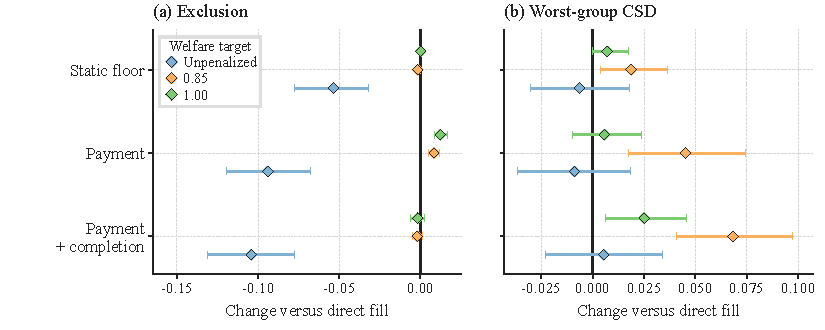
\includegraphics[width=\textwidth]{fig_coverage.pdf}
\caption{Paired effects of changing the allocation rule, relative to direct
greedy fill, on \EvalSeriesN{} held-out Warsaw series. Score weights and feature
definitions stay fixed, but each rule generates its own history and therefore
may produce different later scores. Points are mean paired
differences and bars are 95\% paired percentile-bootstrap intervals. \textbf{(a)}
At the unpenalized score, every alternative rule lowers exclusion and the
intervals exclude zero. At the regularized scores, these effects weaken or reverse.
\textbf{(b)} No kernel yields a statistically detectable improvement in
worst-group deficit; the regularized contrasts mostly worsen it. The
unpenalized replay shows a coverage gain that CSD does not directly measure.}
\label{fig:coverage}
\end{figure}

\paragraph{The payment effect depends on the fitted score.}
Figure~\ref{fig:coverage} and Table~\ref{tab:kernel-intervention} show that, at
the unpenalized score, iterative payment lowers exclusion to
\KernelPaymentOnlyExcl{} and raises welfare
\KernelPaymentOnlyWelfareFactor$\times$. Approval-count completion further
lowers exclusion to \KernelPaymentCompleteExcl{} and raises welfare
\KernelPaymentCompleteWelfareFactor$\times$. Neither CSD contrast is
statistically detectable. At both welfare-regularized scores, payment alone
instead lowers welfare and raises exclusion; completion attenuates the coverage
loss but does not consistently raise welfare. The corresponding payment-based
CSD contrasts worsen. The replay therefore explains one score's coverage
failure. It does not establish that payment protects coverage or fairness in general.

Proposition~\ref{prop:representative} explains why the outcomes can move in
opposite directions. CSD does not record how many distinct voters are served,
so the objective cannot reward the coverage change directly. The fitted sweeps
span \RangeEndowWidth{} and \RangeOutcomeWidth{}
(Appendix Figure~\ref{fig:frontier}), but those widths depend on this corpus, class, and
optimizer. Only the frozen-score replay holds score weights and feature
definitions fixed while changing the allocation rule.

We next compare the fitted classes on this corpus and ask how much of their
performance requires the learned intervention.

\section{What the Warsaw fit changes}
\label{sec:frontier}

\begin{table}[ht]
\centering
\footnotesize
\begin{tabular}{lccc}
\toprule
Rule & Mean worst-group $\csd$ $\downarrow$ & Welfare $\uparrow$ & Exclusion $\downarrow$ \\
\midrule
Recorded outcome & \TestHistoricalCSD & \TestHistoricalWelfare & \TestHistoricalExcl \\
Greedy (approval count) & \TestGreedyCSD & \TestGreedyWelfare & \TestGreedyExcl \\
Greedy (approvals/cost) & \TestGreedyCostCSD & \TestGreedyCostWelfare & \TestGreedyCostExcl \\
\MES{} & \TestMESCSD & \TestMESWelfare & \TestMESExcl \\
\RES{} $(\lambda{=}1)$ & \TestRESCSD & \TestRESWelfare & \TestRESExcl \\
LLMRule (published count score) & \LLMRuleCardCSD & \LLMRuleCardWelfare & \LLMRuleCardExcl \\
\midrule
\multicolumn{4}{l}{\emph{Endowment family (mechanism retained)}} \\
Learned endowment map, no welfare penalty & \EndowCSD & \EndowWelfare & \EndowExcl \\
\midrule
\multicolumn{4}{l}{\emph{Static demographic reference (exploratory, post-lock)}} \\
Four-bracket age lookup & \AgeLookupCSD & \AgeLookupWelfare & \AgeLookupExcl \\
\midrule
\multicolumn{4}{l}{\emph{Outcome family (mechanism discarded)}} \\
Learned, soft target \LearnedHeadFloor & \LearnedHeadCSD & \LearnedHeadWelfare & \LearnedHeadExcl \\
Learned, soft target \LearnedAggrFloor & \LearnedAggrCSD & \LearnedAggrWelfare & \LearnedAggrExcl \\
Learned, no welfare penalty & \LearnedCornerCSD & \LearnedCornerWelfare & \LearnedCornerExcl \\
\bottomrule
\end{tabular}
\caption{Held-out results. The recorded row replays public winner sets; all
other rows are executable counterfactuals. The four reported hand-designed
rules (greedy approvals/cost, \MES{}, and \RES{}$(\lambda{=}0.5,1.0)$) span
$[\HandBandLo, \HandBandHi]$. We replay LLMRule
\citep{thach2026llmrule} without refitting. CSD and exclusion are series-weighted;
welfare is summed. The age lookup is a post-lock exploratory audit, not a
confirmatory or cross-city result.}
\label{tab:main}
\end{table}

The four hand-designed rules cover a narrow range of held-out outcomes
(Appendix Figure~\ref{fig:frontier}). Both learned classes produce results
outside that range. The unpenalized direct-score fit is not the best observed
endpoint: a nearby regularized fit has both lower CSD and higher welfare.



\subsection{Regularization and heterogeneity}

The unpenalized direct-score fit has the largest train--test gap:
\LearnedCornerGap{}, compared with \LearnedHeadGap{} at soft target 1.00. The
target-1.00 fit reduces mean worst-group CSD by \SigHeadDiffAbs{} (95\% CI
\SigHeadCI, raw $p$~\SigHeadP; Holm $p$~\SigHeadHolmP{} in the
\WarsawHolmFamilyN{}-contrast direct-score/endowment/senior-tilt family).
Targets 1.02 and 1.05 show no detectable effect.
Seed spread is \SeedSpread{} at the headline target and grows toward the
aggressive end, as the seed band of Appendix Figure~\ref{fig:frontier} and
Appendix Table~\ref{tab:seeds} both show. The
full sweep and the secondary family of related tests appear in
Appendices~\ref{app:optim} and~\ref{app:stats}.

\paragraph{Ablation and district variation.}
\label{sec:ablation}
Removing cost share, approvals per cost, or carried deficit worsens the
direct-score model in the single-refit comparison. Removing cohort
concentration improves CSD by \AblConcDeltaAbs{}. The model may be exploiting
this proxy, but the ablation does not identify a single cause. When we rescore the same allocations
with age-only or sex-only groups, both learned policies remain below \MES{}
($p\le\PartMaxLearnedP$). These are dependent, secondary exploratory
evaluations, not new fits. The
direct-score policy loses on \PerSeriesLosses{} districts (\LossSeriesList), and
the endowment average also reflects larger wins than losses. Appendix tables
report every ablation, partition, and district result.

\section{Learned endowments on held-out Warsaw elections}
\label{sec:endowment}

The hand-designed \RES{} rollover rule adjusts endowments with one scalar.
Its CSD barely differs from Equal Shares (\TestRESCSD{} versus
\TestMESCSD{}). This result concerns that particular parametrization; it does
not establish that changing endowments is ineffective.

The fitted endowments reach \EndowCSD{}, compared with \TestMESCSD{} for Equal
Shares. The reduction is \EndowSigMESDiffAbs{} (95\% CI \EndowSigMESCI,
raw $p$~\EndowSigMESP; Holm-adjusted $p$~\EndowSigMESHolmP,
\EndowSigMESWins{} series). Welfare falls by
\EndowWelfareCostPct{}, while exclusion falls from \TestMESExcl{} to
\EndowExcl{}. The policy retains the approver-funded payment phase and its
charge accounting because it belongs to the Equal Shares family by
construction. We do not attribute standard priceability or an unweighted
proportionality axiom to the nonuniform endowments or greedy completion.

The published LLMRule count score reaches CSD \LLMRuleCardCSD{} without
refitting. The endowment map's CSD is lower by
\EndowSigLLMRuleCardDiffAbs{} (secondary exploratory $p$~\EndowSigLLMRuleCardP).

\paragraph{Direct scoring has lower CSD at a common soft target.}
The main table compares an unpenalized endowment fit with a welfare-regularized
direct-score fit. These fits use different objectives. In a separate frontier
sweep, we give both classes the same soft target, positive penalty, and number
of generations. Their dimensions, evaluation counts, learned objects, and
features still differ. At target \LearnedHeadFloor{} for both,
learned endowments reach
\MatchedTargetEndowCSD{} against \MatchedTargetDirectCSD{} for direct scores, a
paired difference of \MatchedTargetDiff{} in favor of direct scoring (95\%
interval [\MatchedTargetCILow{}, \MatchedTargetCIHigh{}], secondary exploratory
$p$~\MatchedTargetP,
\MatchedTargetWins{} series). Only exclusion favors the payment-based class,
\MatchedTargetEndowExcl{} against \MatchedTargetDirectExcl{}. This common-target
comparison favors direct scoring on CSD, but it does not identify the effect of
payment because the two policy classes remain structurally different.

\paragraph{Static demographic controls reach lower mean CSD.}
The senior tilt reaches \TiltCSD{} (raw $p$~\TiltP; Holm $p$~\TiltHolmP), the
six-feature map \EndowCSD{}, and a history-free version \StaticTiltCSD{}.
These means do not establish a benefit from temporal memory. We also fit a
four-parameter age lookup on the training split in a post-lock exploratory
analysis. It reaches \AgeLookupCSD{}. In the corrected post-hoc replay, the
six-feature contextual model's CSD minus the lookup's CSD is
\ContextualVsAgeLookupDiff{} (95\% CI \ContextualVsAgeLookupCI,
unadjusted exploratory $p$~\ContextualVsAgeLookupP,
\ContextualVsAgeLookupRecord{} wins/ties/losses),
so we find no statistically detectable series-level difference between the policies.

The lookup has higher exclusion and lower welfare. Exclusion is \AgeLookupExcl{} versus
\EndowExcl{} for the learned map and \TestMESExcl{} for \MES{}; welfare is
\AgeLookupWelfare{} (\AgeLookupWelfareCostPct{} below \MES{}). Multipliers
[\AgeLookupMultipliers] leave almost no endowment for the younger brackets
and concentrate it on the oldest. We use this lookup as an exploratory reference.

Across \EndowNumSeeds{} six-feature fits, held-out CSD ranges from
\EndowSeedLo--\EndowSeedHi{}. In the disjoint-series check, the learned map reaches
\DistrictCVLearnedCSD{} versus \DistrictCVMESCSD{} for \MES{}
(\DistrictCVWins{} wins). However, 18 of the 19 series are Warsaw districts and
the overlapping training folds are not independent replications. Appendix
Tables~\ref{tab:district-cv} and~\ref{tab:district-bound} report all folds and
the coefficient-box sensitivity. Appendix~\ref{app:transfer} contains the
no-refit non-Warsaw stress set.

\section{External transfer tests}
\label{sec:sequential-transfer}

We locked two studies before opening their held-out ballots: learned priority
and endowments evaluated on projected support sets. Each lock fixes the corpus,
fitted weights, rule, and decision thresholds. The opening receipts record the
lock digests. The native replay below is a separate post-hoc analysis.
Appendix~\ref{app:external} gives the artifacts and conditions.

The corrected post-hoc replay of the first locked study, learned priority
inside Equal Shares, remains \emph{falsified}. The temporal city-macro CSD
contrast misses the threshold, some city estimates do not point downward, and
priorities change fewer allocations than matched endowments. Welfare and
exclusion safeguards pass, but the study finds no stable fairness benefit.

The second test applies the fixed learned endowments in two new cities. We
convert cumulative and ordinal ballots to projected support sets, keeping the
listed projects but discarding point magnitudes and ranks. The lock covers
\ExternalElectionN{} elections across \ExternalSeriesN{} series;
\ExternalScoreN{} elections are scored. It uses three fixed seeds $1,2,42$ and equal-city aggregation.

\begin{figure}[t]
\centering
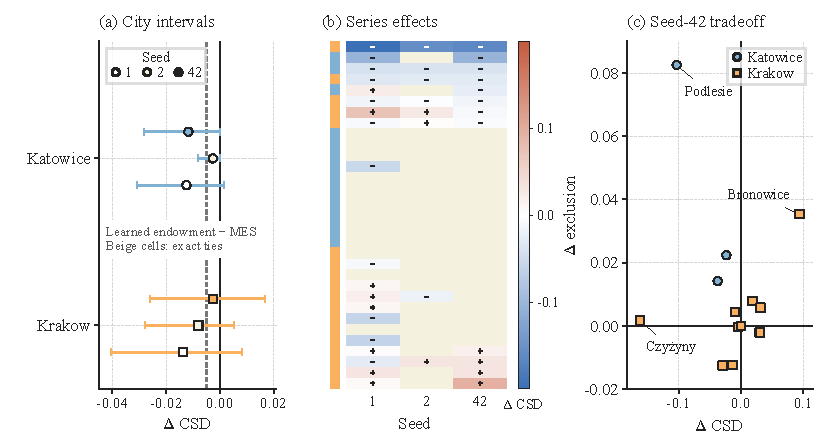
\includegraphics[width=\textwidth]{fig_external.pdf}
\caption{Fresh-city results over projected support sets
($n=\ExternalSeriesN{}$ series). The endowment map changes allocations on
\ActuatingSeries{} series. \textbf{(a)} Endowment-minus-\MES{} city means use
95\% paired bootstrap intervals. The three fixed-seed city-macro effects are
\ExternalSeedOneMacro{}, \ExternalSeedTwoMacro{}, and
\ExternalSeedFortyTwoMacro{}. At the primary seed, the Holm-adjusted $p$ values
are \ExternalKatowicePrimaryHolmP{} for Katowice and
\ExternalKrakowPrimaryHolmP{} for Krakow. \textbf{(b)} Per-series effects use
beige for exact ties, $+/-$ for sign, and the side strip for city. \textbf{(c)}
Primary-seed CSD and exclusion changes are
descriptive, not causal: negative CSD change favors learned endowments, while
positive exclusion change is adverse. Projection discards cumulative point
magnitude and ordinal rank.}
\label{fig:external}
\end{figure}

The endowment map changes an allocation on only \ActuatingSeries{} series.
\ActuatingInert{} series reproduce Equal Shares exactly. Conditional on an
allocation change, the primary-seed CSD contrast is \ActuatingMeanSubset{},
compared with \ActuatingMeanAll{} across all series
(\ActuatingWins{} wins and \ActuatingLosses{} losses). The corresponding
conditional effects over all seeds lie in
[\ActuatingMeanSubsetLo, \ActuatingMeanSubsetHi]. Because this subset is defined
by the observed outcome, the comparison is descriptive and does not alter the
locked test. On most fresh-city series, the fitted intervention leaves the
allocation unchanged. These exact ties also help explain why the
Katowice interval reaches \ExternalKatowicePrimaryCIHigh{}.

Across all series, endowment-minus-\MES{} estimates are negative in both cities
for every seed. Equal-city macro changes are \ExternalSeedOneMacro{},
\ExternalSeedTwoMacro{}, and \ExternalSeedFortyTwoMacro{}. The primary result
contains \ExternalPrimaryWins{} wins, \ExternalPrimaryTies{} exact ties, and
\ExternalPrimaryLosses{} losses. The all-series effect is directionally
favorable but seed-sensitive.

The lock evaluates eight conditions. Direction, macro-effect, welfare, and
actuation pass. The failures are city-level uncertainty, primary Holm significance,
the exclusion safeguard, and seed spread. The primary intervals extend to
\ExternalKatowicePrimaryCIHigh{} in Katowice and
\ExternalKrakowPrimaryCIHigh{} in Krakow, while the Holm-adjusted $p$ values are
\ExternalKatowicePrimaryHolmP{} and \ExternalKrakowPrimaryHolmP{}. Katowice
exclusion increases by \ExternalKatowiceSeedOneExclDelta{} and
\ExternalKatowiceSeedFortyTwoExclDelta{} at seeds 1 and 42. The locked decision
is therefore falsified. The small number of allocation changes helps explain
the uncertainty, but it does not establish successful generalization.

\paragraph{Native approval ballots, without projection.}
Gdynia and \L{}\'od\'z provide a post-hoc, no-refit replay on
\CrossCitySeriesN{} native-approval series. The frozen Warsaw fit gives
\CrossCityAllLearned{} versus \CrossCityAllMES{} (difference
\CrossCityAllDiff{}; 95\% paired interval [\CrossCityAllCILow{},
\CrossCityAllCIHigh{}], $p$~\CrossCityAllP{}, \CrossCityAllWins{} series);
neither city differs detectably from zero. The map exactly matches Equal Shares
on \CrossCityInertN{} series, whose median is
\CrossCityMedianProjectsInert{} projects per scored election versus
\CrossCityMedianProjectsActive{} when it acts. The estimated effect remains
near zero across the reported granularity grid (Table~\ref{tab:crosscity}).
Thresholds change sample size and composition, so this grid does not isolate
the role of low actuation.

Projection changes ballot lengths and approval overlap, both of which are map features. The
native inert rate (\CrossCityInertN{}/\CrossCityAllSeriesN{}) nearly matches the
projected study (\ActuatingInert{}/\ExternalSeriesN{}); median project counts
are \ExternalMedianProjects{} under projection and \WarsawMedianProjects{} in
Warsaw. Series with fewer projects are more likely to have unchanged
allocations. Other differences between cities remain unresolved.

\section{Related work}
\label{sec:related}

Research on PB studies proportionality and repeated representation
\citep{aziz2015jr,peters2020welfarism,lackner2020perpetual,elkind2023temporal}.
Learned systems fit project-scoring aggregation rules
\citep{fairstein2024learningpb} or evolve executable priority programs
\citep{thach2026llmrule}; mixed rules alter \MES{} budgets after project
selection \citep{baychkov2026mixed}. We learn endowments before project
selection and, in a separate replay, fix the project-score parameters while
changing the allocation rule. We do not claim to introduce learned PB rules
or nonuniform \MES{} budgets. Our audit also connects to mechanism-informed learning
\citep{maruo2026mechanism} and tests of reward hacking
\citep{skalse2022defining}; Appendix~\ref{app:related} details the PB comparison.

\section{Limitations}

\paragraph{Evidence scope.} The corrected Warsaw replay provides within-city
evidence, not a fresh holdout test. The projected-support study covers \ExternalSeriesN{} series in two new
cities, but changes few allocations and has seed sensitivity, city-level
uncertainty, and increases in exclusion. It does not establish transfer to
native ballots. The post-hoc native replay finds no detectable series-level
difference and leaves allocations unchanged on \CrossCityInertN{} series. All external
cities are Polish. Both locked studies fail, and the native replay is not
confirmatory. The post-lock age lookup also prevents us from attributing the
Warsaw reduction to learned context.

\paragraph{Identification and deployment limits.} The frontier compares
fitted classes with different learned objects and features. It cannot isolate
the causal effect of the payment rule. Weight vectors are not identifiable,
so we do not interpret individual coefficients. Direct scoring has no
proportionality axiom. The frozen-score replay explains one Warsaw coverage
failure, not a general safeguard. Fixed ballots also cannot reveal voters'
strategic responses. Administrative age-by-sex groups describe voters
incompletely. Changing the partition changes the objective, and demographic
missingness may be nonrandom
(Appendix~\ref{app:corpus}).

\section{Conclusion}

CSD measures group spending shares, not the number of voters served.
At the fixed unpenalized score, payment reduces exclusion
from \KernelDirectExcl{} to \KernelPaymentOnlyExcl{} and raises welfare to
\KernelPaymentOnlyWelfareFactor$\times$ the direct-score value. Completion
brings exclusion to \KernelPaymentCompleteExcl{} and welfare to
\KernelPaymentCompleteWelfareFactor$\times$. Neither CSD contrast is
statistically detectable at this score, and both worsen CSD at the two
regularized targets. Reporting coverage alongside CSD makes this difference visible.

The fixed endowment map leaves allocations unchanged on
\CrossCityInertN{}/\CrossCitySeriesN{} native-approval series. In Warsaw, it lowers CSD but costs \EndowWelfareCostPct{}
in welfare. A post-lock age lookup reaches \AgeLookupCSD{} with worse exclusion
and welfare. Both locked studies fail, including the projected-support
city-level uncertainty criterion. The post-hoc native replay finds no
detectable difference. Neither a benefit from learned context nor transfer is
established. Report objective value, coverage, and allocation changes
separately. Replay fixed score parameters across allocation rules to help
distinguish the score's contribution from the rule's.

\newpage
\section*{Reproducibility statement}

Manuscript macros and tables are checked against authenticated stored results.
The primary Warsaw results use the corrected v2 fit and evaluation artifacts;
the post-lock contextual comparison uses a separately recorded paired audit.
These are corrected post-hoc replays, not fresh untouched holdout tests.
Appendix~\ref{app:corpus} describes the corrections and retained evidence.
The statistical figures use the same stored outputs. The public corpus
\citep{stolicki2020pabulib} is split and frozen before
fitting. A 415-file integrity manifest pins the frozen Warsaw, multi-city, and
native cross-city corpus files to official Pabulib commit \texttt{2f4321f}
(the artifact records the full hash), and every file matches the recorded size
and SHA-256 digest. Both locked studies and the separate native replay write a
manifest for their held-out corpus; only the first two have pre-opening
protocol locks.

Run JSONs record every fitting seed. Analysis scripts or companion manifests
fix the resampling seeds. The optimizer is a \OptimizerLines{}-line CMA-ES
implementation that depends only on NumPy. None of the experiments requires a
GPU, network connection, or API key. Three verification scripts reproduce the
reference replay and the endowment/direct-score containments
(Section~\ref{sec:containment}). One of these checks found the ballot-counting
defect described above.

\section*{Ethics statement}

This study reuses a public participatory-budgeting corpus and collects no new
human-subject data. The fairness analysis uses age and sex fields released with
the ballots. These administrative categories are incomplete descriptions of
voters and poor substitutes for communities. We report only aggregate group
outcomes and do not infer missing demographic attributes. The learned rules are
research prototypes, not deployment recommendations.

The worst-served group is nearly fixed in this corpus. It is men aged 60 or
older in \WorstCohortSeniorMale{} series, voters aged 60 or older in
\WorstCohortSenior{}, and men of some age in \WorstCohortMale{}. Minimizing the
largest deficit therefore usually creates pressure to redirect spending toward
older men in these data.

This pattern does not show that older men are disadvantaged more broadly. CSD
compares the attributed spending attracted by a group's ballots with its share
of turnout. Older voters in this corpus submit shorter ballots, which attract
less attributed spending under the metric. Because the maximization usually
selects the same demographic group, the objective also behaves more like a
single-group deficit than the notation suggests. Any deployment would require
an explicit local choice of groups and attribution rules. Our partition should
not be inherited by default.

\section*{AI use statement}

Generative AI tools were used during hypothesis refinement, study design,
implementation, data preparation, result interpretation, proof checking,
literature search, and manuscript editing. The authors verified the resulting
claims against the code, stored outputs, proofs, and cited sources and accept
responsibility for the submission.

\bibliography{refs}
\bibliographystyle{iclr2027_conference}

\appendix
% Appendix for the ICLR 2027 submission.
% Included from main.tex after \appendix. Every number here resolves to a macro
% in numbers.tex or to a table generated from results/.

\clearpage
\section{Notation}
\label{app:notation}

\begin{center}
\small
\begin{tabular}{ll}
\toprule
Symbol & Meaning \\
\midrule
$I_t = (P_t, c_t, b_t, N_t, A_t)$ & edition $t$: projects, costs, budget, voters, ballots \\
$A_t(i) \subseteq P_t$ & the approval ballot of voter $i$ \\
$A_t(p) \subseteq N_t$ & the approvers of project $p$ \\
$N_t^{\mathrm{cov}}\subseteq N_t$ & voters with the demographics needed for the group ledger \\
$G$ & the group partition (age $\times$ sex cells the ballots record) \\
$g_t$ & covered members of group $g$ among edition-$t$ voters \\
$W_t \subseteq P_t$ & the funded set, $c_t(W_t) \le b_t$ \\
$u_t(g)$ & money attributed to $g$ (Definition~\ref{def:csd}) \\
$e_t(g)$ & entitlement of $g$, its share of money spent \\
$\csd_T(g)$ & cumulative share deficit of $g$ after $T$ editions \\
$\mathcal{H}_{t-1}$ & history available to a policy entering edition $t$ \\
$\beta_i$ & endowment of voter $i$; uniform $\beta_i = b_t/|N_t|$ is \MES \\
$w \in \mathbb{R}^{6}$ & endowment-family weights \\
$v \in \mathbb{R}^{5}$ & outcome-family weights \\
$\rho$ & Equal Shares price level at which a project is bought \\
$\kappa$ & largest endowment multiple, $\max_i \beta_i |N_t| / b_t$ \\
$\tau, \mu$ & soft welfare target and its penalty weight \\
$\lambda$ & rollover intensity of \RES \\
\bottomrule
\end{tabular}
\end{center}

\section{Corpus and splits}
\label{app:corpus}

\paragraph{Construction.}
We build the fitting corpus from the frozen Pabulib snapshot
\citep{stolicki2020pabulib}. We keep nonempty approval elections with recorded
winners, at most $300{,}000$ voters, and demographic data on at least half
of the ballots. We then group elections by (city, district). A group qualifies
as a \emph{series} if its longest consecutive run contains at least three
editions. The corpus contains
\NumSeriesTotal{} series and \PrimaryElectionN{} elections, comprising
\PrimaryBallotN{} ballots and \PrimaryProjectN{} projects from
\PrimaryYearLo--\PrimaryYearHi. We exclude the Warsaw citywide contest and a
Wawer subunit because both aggregate ballots that already appear in the
district series.

\paragraph{Fitting corpus versus available corpus.}
We fit the headline Warsaw weights only on the primary corpus above. Applying
the same filter to the complete public repository admits many additional
series, mostly outside Warsaw, including histories in Gdynia and \L{}\'od\'z
that are long enough for the temporal protocol. An earlier version used an
incomplete local download and incorrectly attributed its limited coverage to
the public data. We corrected the download without refitting the headline
weights. The locked projected-support study uses separate pooled-temporal
fits trained on pre-2023 histories from Gdynia, Warsaw, and \L{}\'od\'z. For
the post-hoc native-approval replay, we use the frozen Warsaw headline fit.
We report no fit on the complete corpus.

\paragraph{Corrected-result lineage.}
The primary Warsaw results come from a saved corrected replay with duplicate
project tokens removed within each ballot and a deterministic project order.
Canonicalization removes one repeated approval token in Wola 2021; no ballot
is removed. The corrected corpus contains 6,577,175 approval tokens across
\PrimaryBallotN{} ballots. We retain the original artifacts and authenticate
the corrected fit and evaluation records separately. Because the original
results had already been inspected, the corrected Warsaw and first multi-city
analyses are post-hoc replays, not new untouched holdout tests. The first
multi-city decision remains \emph{falsified}. The projected-support external
study and the native-approval replay retain their separate recorded lineages.
The manuscript reconstruction uses saved estimates and intervals; it does not
rerun fitting or statistical tests.

\paragraph{Missing demographics.}
Every ballot contributes to the \emph{allocation}. When age or sex is missing,
the approvals still affect funding, but the ballot cannot enter the cohort
ledger because we cannot assign it to a group. Project scores therefore count
all ballots, while the fairness ledger counts only covered ballots. Confusing
these counts caused the defect described in Appendix~\ref{app:containment}.
The filter requires demographics on half of an election's ballots. We do not
model why fields are missing. If coverage depends on age or sex, for example
through the voting channel, the ledger represents a nonrandom subsample, and
that selection affects every deficit, entitlement, and $\csd$ value. We do
not test this missingness assumption.

\paragraph{Splits.}
The temporal split fits on editions through 2022 and evaluates on 2023--2025:
\SplitTrainEditions{} training editions and \SplitTestEditions{} held-out
editions across \EvalSeriesN{} series. The \L{}\'od\'z citywide contest enters
the fitting corpus only in 2023 and thus has no training editions. We exclude
that series from the temporal split and use it for the no-refit city-out replay
in Section~\ref{sec:transfer}. The district series available in the complete
repository are held out entirely for Appendix~\ref{app:external}. We use no
\L{}\'od\'z data to fit the primary temporal policies. Repeated analysis of
the citywide series limits its role to a descriptive transfer case rather than
external validation.

A separate five-fold disjoint-series check uses the complete history of every
series. We hold \L{}\'od\'z out in one fold and include it in training in the
other four. This check evaluates disjoint series, so it tests neither temporal
nor Warsaw-to-\L{}\'od\'z transfer. We save each split to disk and reload it
to keep the boundaries fixed across runs.

Here, held-out editions are excluded from fitting the shared weight vector.
Allocation still uses the edition-$t$ ballots, project costs, and budget once
they are available. The recorded winner set is never a policy feature. Each
counterfactual policy replays a series in order and updates
$\mathcal{H}_{t}$ using only its own selected outcome after scoring edition $t$.

\section{Feature definitions}
\label{app:features}

Every feature is dimensionless. Setting $w=0$ in the endowment parametrization
recovers \MES. In the outcome family, $v=e_1$ and $v=e_2$ recover the two
baselines, while the zero vector does not. Let $n = |N_t|$, $b = b_t$, and
write $\bar{\ell}$ for the mean ballot length over covered voters.

\paragraph{Endowment family.}
For group $g$ with carried deficit $D_{t-1}(g) = \sum_{\tau<t}(e_\tau(g) - u_\tau(g))$
and carried entitlement $E_{t-1}(g) = \sum_{\tau<t} e_\tau(g)$:
\begin{align*}
f_1(g) &= \frac{\max(0, D_{t-1}(g))}{|g_t| \cdot (b/n)}
  &&\text{deficit per capita, in units of the base endowment}\\
f_2(g) &= \mathrm{clip}\!\left(\frac{D_{t-1}(g)}{E_{t-1}(g)},\, -1,\, 1\right)
  &&\text{signed deficit as a fraction of entitlement owed}\\
f_3(g) &= \frac{|g_t|}{n_{\mathrm{cov}}} - \frac{1}{|G|}
  &&\text{size relative to an equal split}\\
f_4(g) &= \frac{\bar{\ell}_g}{\bar{\ell}} - 1
  &&\text{ballot length relative to the electorate}\\
f_5(g) &= \frac{\bar{c}_g}{\bar{c}} - 1
  &&\text{mean cost per approval, relative}\\
f_6(g) &= \cos\!\big(\phi_g, \phi_{\mathrm{all}}\big) - \overline{\cos}
  &&\text{approval-profile overlap, mean-centred over groups}
\end{align*}
Here $\phi_g$ is the vector of per-project approval frequencies within $g$.
History enters only through $f_1$ and $f_2$. A voter without recorded
demographics receives raw endowment $b/n$. For a covered voter,
$w = \lambda e_1$ gives raw endowment
$b/n + \lambda \max(0, D_{t-1}(g))/|g_t|$. The common budget normalization then
recovers \RES{} exactly.

\paragraph{Outcome family.}
For project $p$ with $\mathrm{sh}(p) = |A_t(p)|/n$ counted over \emph{all}
ballots and $\mathrm{cs}(p) = c_t(p)/b$:
\begin{align*}
\varphi_1(p) &= \mathrm{sh}(p) &&\text{approval share} \\
\varphi_2(p) &= \frac{\mathrm{sh}(p)/\mathrm{cs}(p)}{\max_q \mathrm{sh}(q)/\mathrm{cs}(q)}
  &&\text{approvals per unit cost, normalized to } [0,1] \\
\varphi_3(p) &= \mathrm{cs}(p) &&\text{cost share} \\
\varphi_4(p) &= \sum_{g} \hat{w}_g \cdot
  \frac{n_{t,g}(p)}{n_t^{\mathrm{cov}}(p)}
  &&\text{support drawn from lagging groups} \\
\varphi_5(p) &= \sqrt{\frac{\sum_g \big(s_g(p) - 1/|G|\big)^2}{1 - 1/|G|}}
  &&\text{concentration of support across groups}
\end{align*}
If at least one group has a positive deficit, the weights satisfy
$\hat{w}_g \propto \max(0, D_{t-1}(g))$ and sum to one. Otherwise, all weights
are zero. The term $s_g(p)$ is the
share of $p$'s covered approvers in $g$. Only $\varphi_4$ uses history. A ratio
over covered approvers is set to zero when the project has no covered approver.
Setting $v=e_1$ recovers greedy approval count, and $v=e_2$ recovers greedy
approvals per unit cost.

The supporter-composition diagnostic in Section~\ref{sec:theory} uses
$q_{t,g}(p)$ for group $g$'s share among the demographically covered approvers
of project $p$, and $s_{t,g}=|g_t|/\sum_h |h_t|$ for its share among covered
voters. We report
\[
\operatorname{TV}_t(p)=\frac{1}{2}\sum_g
  \left|q_{t,g}(p)-s_{t,g}\right|,
\]
as a raw-cost-weighted average over funded projects. We compute this quantity
only on held-out editions after replaying each policy's training prefix.
The optimizer uses this descriptive measure neither as a feature nor as an
objective.

\section{Mechanism implementation}
\label{app:mechanism}

\begin{algorithm}[ht]
\caption{Equal Shares with general endowments, and completion}
\label{alg:mes}
\begin{algorithmic}[1]
\Require instance $(P, c, b, N, A)$, endowments $\beta \ge 0$
\State $W \gets \emptyset$;\; $\mathcal{A} \gets \{p : A(p) \neq \emptyset,\, c(p) > 0\}$
\While{$\mathcal{A} \neq \emptyset$}
  \ForAll{$p \in \mathcal{A}$}
    \If{$\sum_{i \in A(p)} \beta_i < c(p)$} \State $\mathcal{A} \gets \mathcal{A} \setminus \{p\}$ \Comment{never affordable; endowments only shrink}
    \Else \State $\rho_p \gets \min\{\rho : \sum_{i \in A(p)} \min(\beta_i, \rho) \ge c(p)\}$
    \EndIf
  \EndFor
  \State \textbf{if} $\mathcal{A} = \emptyset$ \textbf{then break}
  \State $p^\star \gets \arg\min_{p \in \mathcal{A}} \rho_p$ \Comment{ties by ascending cost, then id}
  \State $\beta_i \gets \beta_i - \min(\beta_i, \rho_{p^\star})$ for $i \in A(p^\star)$
  \State $W \gets W \cup \{p^\star\}$;\; $\mathcal{A} \gets \mathcal{A} \setminus \{p^\star\}$
\EndWhile
\State \Comment{completion: Equal Shares is not exhaustive, so spend the remainder}
\State $r \gets b - c(W)$
\ForAll{$p \notin W$ with $A(p)\neq\emptyset$ in descending $|A(p)|$,
  ties by ascending $c(p)$, then id}
  \If{$c(p) \le r$} \State $W \gets W \cup \{p\}$;\; $r \gets r - c(p)$ \EndIf
\EndFor
\State \Return $W$
\end{algorithmic}
\end{algorithm}

Completion spends the remaining budget by approval count and falls outside the
payment rule. It accounts for the nonzero uniform Equal Shares value in
Table~\ref{tab:infeasible}; the learned-endowment value uses the same uniform
reference floor, not the learned cap. We find $\rho_p$ in one pass over the
sorted approver endowments. The absolute tolerance is $10^{-9}$ for aggregate
affordability and $10^{-12}$ for water-filling breakpoints.

\begin{algorithm}[ht]
\caption{Outcome family, with an optional support floor}
\label{alg:outcome}
\begin{algorithmic}[1]
\Require instance, weights $v$, optional $\kappa$
\State $E \gets \{p : A(p) \neq \emptyset\}$
\If{$\kappa$ given} \State $E \gets \{p \in E : |A(p)|/n \ \ge\ c(p)/(\kappa b)\}$ \EndIf
\State $W \gets \emptyset$;\; $r \gets b$
\ForAll{$p \in E$ in descending $v^{\top}\varphi(p)$, ties by ascending
  $c(p)$, then id}
  \If{$c(p) \le r$} \State $W \gets W \cup \{p\}$;\; $r \gets r - c(p)$ \EndIf
\EndFor
\State \Return $W$
\end{algorithmic}
\end{algorithm}

\section{Optimization}
\label{app:optim}

We fit both arms with the same self-contained CMA-ES implementation. It uses
\OptimizerLines{} lines of NumPy and runs without a GPU or dependencies on
SciPy, cma, or PyTorch.

\begin{table}[ht]
\centering\small
\begin{tabular}{lcc}
\toprule
 & Endowment arm & Outcome arm \\
\midrule
Search dimension & 6 & 5 \\
Population $\lambda = 4 + \lfloor 3\ln d\rfloor$ & 9 & 8 \\
Parents $\mu = \lfloor \lambda/2 \rfloor$ & 4 & 4 \\
Initial step $\sigma_0$ & 0.4 & 0.4 \\
Generations & 30 (headline); 25 (frontier/stability) & 25 \\
Objective evaluations & 271 headline; 225 frontier; 226 stability & 200 per target \\
Weight box & $[-10, 10]$ & $[-10, 10]$ \\
Penalty weight $\mu$ & 0 headline; 0/2.0 frontier & 0/2.0 frontier \\
Seeds & 42, 1, 2 & 42, 1, 2, 3 \\
Corrected-run wall clock & Not recorded & Not recorded \\
\bottomrule
\end{tabular}
\caption{Optimizer settings. In Section~\ref{sec:ablation}, ``same optimization
budget'' means 25 generations with population 8, as in the frontier fits used
for comparison. The original fits used \computehardware, without a GPU.
The corrected fit artifacts do not record elapsed times, so we do not report
corrected-run wall-clock ranges. Endowment evaluation replays iterative Equal
Shares; the outcome arm uses a greedy pass.}
\end{table}

The headline endowment fit and its two additional seeds use different numbers
of generations. Their range gives an informal check of optimizer stability,
with no estimate of variance under matched optimization budgets.

Each of the five primary disjoint-series fits uses 25 generations and the
coefficient box $[-10,10]$. All five reach the boundary. We therefore ran a
matched post hoc set with box $[-40,40]$ and separate artifact tags, but four
of the wider fits also reach their boundary. Table~\ref{tab:district-bound}
compares held-out outcomes. These results support neither coefficient
interpretation nor a claim of independent replication.

We leave the features unstandardized. Election-level ratios are dimensionless,
and the two history features retain their longitudinal scale. No fit uses a
restart. We initialize the means at the hand-designed references \RES$(1)$
for endowments and greedy approvals-per-cost for outcomes. Because CMA-ES need
not return its initial mean as a candidate, we replay and report every
baseline separately.

\paragraph{Why distinct soft welfare targets can return identical policies.}
The penalty is $\mu \max(0, \tau - \text{ratio})$. When the unconstrained
optimum exceeds $\tau$, it incurs no penalty and remains optimal. If $\tau$
exceeds every attainable welfare ratio, each candidate incurs
$\mu(\tau - \text{ratio})$. Increasing $\tau$ then adds the same constant to
every objective value, leaving the minimizer unchanged. The trade-off changes
only in the intermediate regime. This formulation explains the identical rows
in Table~\ref{tab:endowfrontier} without implying a failed search.

We use $\tau=1$ as the headline outcome-arm operating point because its
training target equals \MES{} approval-count welfare. Neither this choice nor
the penalty weight $\mu=2$ was preregistered. Table~\ref{tab:endowfrontier}
reports the full tested target grid. The headline selection remains
exploratory.

\section{Containment verification}
\label{app:containment}

\begin{table}[ht]
\centering\small
\begin{tabular}{lccc}
\toprule
Identity & Scope & Tolerance & Result \\
\midrule
$w = \mathbf{0} \Rightarrow \MES$ & \NumSeriesTotal{} series & exact & max $|\Delta| = 0$ \\
$w = \lambda e_1 \Rightarrow \RES(\lambda)$, 5 values & \NumSeriesTotal{} series & exact & max $|\Delta| = 0$ \\
$v = e_1 \Rightarrow$ greedy-by-count & \PrimaryElectionN{} elections & set equality & \PrimaryElectionN{}/\PrimaryElectionN{} \\
$v = e_2 \Rightarrow$ greedy-by-cost & \PrimaryElectionN{} elections & set equality & \PrimaryElectionN{}/\PrimaryElectionN{} \\
environment vs.\ frozen replay & \NumSeriesTotal{} series, 3 rules & $5\times10^{-4}$ & \NumSeriesTotal{}/\NumSeriesTotal{} \\
\bottomrule
\end{tabular}
\end{table}

The first run failed the third identity on 4 of \PrimaryElectionN{} elections.
The learned score counted approvals only on demographically covered ballots,
while the deployed rule counted every ballot. These counts agree when coverage
is complete, but partial coverage can change the project order. We corrected
the implementation by separating allocation counts from ledger counts
(Appendix~\ref{app:corpus}). The containment test found the defect, which code
review had not detected. Without that check, the wrong counts could have
produced plausible results.

\section{Proof of Proposition~\ref{prop:support}}
\label{app:proof}

\begin{proof}
Let $W_{\mathrm{pay}}$ be the outcome of Algorithm~\ref{alg:mes} before
completion, and let $p \in W_{\mathrm{pay}}$ be bought at price level $\rho$.
By the purchase rule, $p$ enters $W_{\mathrm{pay}}$
only when its approvers can cover its cost at that level:
\[
\sum_{i \in A(p)} \min(\beta_i^{(p)}, \rho) \;\ge\; c(p),
\]
where $\beta^{(p)}$ are the endowments remaining when $p$ is bought. Endowments
are non-increasing along the run, since each purchase only subtracts, so
$\beta_i^{(p)} \le \beta_i$ for the initial vector $\beta$. Also
$\min(x, \rho) \le x$. Chaining these,
\[
c(p) \;\le\; \sum_{i \in A(p)} \min(\beta_i^{(p)}, \rho)
      \;\le\; \sum_{i \in A(p)} \beta_i^{(p)}
      \;\le\; \sum_{i \in A(p)} \beta_i .
\]
Now suppose $\beta_i \le \kappa\, b/|N|$ for every $i$. Then
$\sum_{i \in A(p)} \beta_i \le |A(p)| \cdot \kappa b / |N|$, and combining with
the display above gives $c(p) \le |A(p)| \kappa b / |N|$, i.e.
$|A(p)|/|N| \ge c(p)/(\kappa b)$, which is the claim.
\end{proof}

The bound is attained when every approver of $p$ still holds exactly
$\kappa b/|N|$ and spends the full amount on $p$, as can happen when none has
paid for an earlier winner. Otherwise the bound is generally slack. Under the
stated cap, the proposition restricts payment-phase purchases but does not
determine a fitted policy's choices. Section~\ref{sec:identification} tests that
region constraint separately and finds that it does not reproduce the
mechanism.

\section{Representative support: proof and executable check}
\label{app:degeneracy}

\begin{proof}[Proof of Proposition~\ref{prop:representative}]
For a fixed group $g$, Definition~\ref{def:csd} and the definitions of
$q_{t,g}(p)$ and $E_g$ give the following, where
$\omega_{t,p,g}=c_t(p)s_{t,g}/E_g$ and
$r_{t,p,g}=q_{t,g}(p)/s_{t,g}$:
\begin{align*}
\csd_T(g)
&= 1-\frac{\sum_t\sum_{p\in W_t}c_t(p)q_{t,g}(p)}{E_g} \\
&= 1-\sum_t\sum_{p\in W_t}
  \frac{c_t(p)s_{t,g}}{E_g}\frac{q_{t,g}(p)}{s_{t,g}}
 = 1-\sum_t\sum_{p\in W_t}\omega_{t,p,g}r_{t,p,g}.
\end{align*}
Because
$\sum_{t,p}\omega_{t,p,g}=\sum_t c_t(W_t)s_{t,g}/E_g=1$,
\[
|\csd_T(g)|
=\left|\sum_{t,p}\omega_{t,p,g}(1-r_{t,p,g})\right|
\leq\sum_{t,p}\omega_{t,p,g}|1-r_{t,p,g}|
\leq\epsilon.
\]

For the construction, let the positive rational group shares be $(s_g)_g$ and choose a
positive integer $m$ such that every $m s_g$ is an integer. Choose a larger
electorate size $n$ with every $n s_g$ integral and $m/n\leq\delta$. Create one
project of cost $b$, approved by exactly $m s_g$ voters from each group, and a
budget-feasible dummy project, also of cost $b$, approved by every other
voter. Fund only the representative project; it exhausts the budget, so the
dummy remains unfunded. Its approver composition is $q_g=s_g$, so the identity
gives $\csd(g)=0$ for every group. Exactly $m$ of $n$ voters approve a funded
project, hence exclusion is $1-m/n\geq1-\delta$.
\end{proof}

The executable construction uses \DegGroups{} equal groups. We keep one
supporter per group and increase the electorate, evaluating each case with the
same \texttt{group\_outcome},
\texttt{cumulative\_share\_deficit}, and \texttt{exclusion\_rate} functions used
in the experiments.

\begin{table}[ht]
\centering\small
\begin{tabular}{rrrr}
\toprule
Voters & Winner supporters & Worst $|\csd|$ & Exclusion \\
\midrule
\DegEightyVoters & \DegSupporters & \DegEightyCSD & \DegEightyExcl \\
\DegTwoHundredVoters & \DegSupporters & \DegTwoHundredCSD & \DegTwoHundredExcl \\
\DegFourHundredVoters & \DegSupporters & \DegFourHundredCSD & \DegFourHundredExcl \\
\DegEightHundredVoters & \DegSupporters & \DegEightHundredCSD & \DegEightHundredExcl \\
\bottomrule
\end{tabular}
\caption{Representative-support construction from
\texttt{iclr\_degeneracy.py}. CSD remains exactly zero in the production ledger
as exclusion approaches one. This construction tests the metric's limits. It
is neither a fitted result nor a candidate policy.}
\label{tab:degeneracy}
\end{table}

\begin{figure}[tb]
\centering
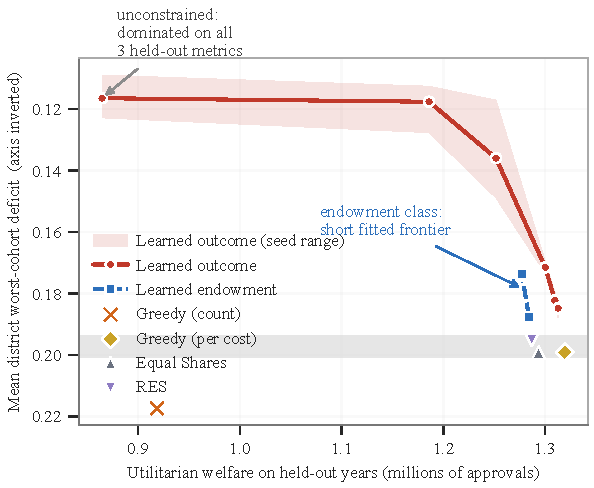
\includegraphics[width=0.72\textwidth]{fig_frontier.pdf}
\caption{Held-out fairness--welfare results for the fitted policy classes. The
grey band covers four hand-designed rules: greedy approvals/cost, \MES{}, and
\RES{}$(\lambda{=}0.5,1.0)$. Its width is \HandBandWidth. Both learned classes
extend beyond the band. Direct scores span \RangeOutcomeWidth{} (red, with
variation across \NumSeeds{} seeds), while learned endowments span
\RangeEndowWidth{} (blue). The classes learn different objects from different
features, so this comparison cannot identify the causal effect of the payment
rule. Mild regularization improves both fairness and welfare over the
unpenalized direct-score point.}
\label{fig:frontier}
\end{figure}

\section{Statistical methodology}
\label{app:stats}

We use the \emph{series} as the inferential unit. Editions within a district
share a project pool and electorate, and the districts themselves belong to
one city. The intervals describe dispersion across districts in this corpus.
They cannot remove common-city shocks or support city-level population
inference. For each policy contrast, we first calculate the difference in
held-out worst-group $\csd$ within each series, then take an equally weighted
mean across series. The reported $2.5$--$97.5$ paired percentile-bootstrap
interval uses $10{,}000$ resamples of these series pairs.

The exact paired test enumerates all $2^{\EvalSeriesN}$ sign assignments of the
series differences under the null. It reports the two-sided fraction whose
absolute mean is at least as large as the absolute observed mean. The test assumes
sign-exchangeable paired differences under the null and treats neither
elections nor voters as independent replicates. We display values below $0.001$
as $p<0.001$. A ``win'' is a series with a negative difference. We report wins
alongside the mean because large improvements in a few series can lower that
mean.

In the disjoint-series analysis, the pooled 19-series mean, win count, and
paired bootstrap interval are descriptive because all series in a held-out
fold share one fitted map. As a sensitivity check, we average the paired
effects within each fold and enumerate all $2^5$ sign assignments of the five
fold means. The fold-block $p$-value has a minimum two-sided resolution of
$0.0625$. These five fits use overlapping training sets and cannot count as
independent replications. This analysis also uses each series' complete
history, so it tests neither temporal nor cross-city transfer.

We apply Holm--Bonferroni correction to the \WarsawHolmFamilyN{} focal held-out
Warsaw comparisons reported in the main text: direct scoring against \MES{},
learned endowments against \MES{}, and the senior tilt against \MES{}. The full
welfare-target grid, closest-prior comparison, matched-target check,
allocation-kernel intervention, and three group partitions remain secondary
exploratory analyses and are unadjusted unless a separate protocol states
otherwise. The partition analyses re-score the same fitted policies, which
makes them dependent. Neither the focal contrasts nor the frozen-score
intervention was preregistered. Adjusting the values controls multiplicity
within this reported family, but the evidence remains exploratory.
In the post-lock audit, the age lookup changes CSD relative to the senior tilt
by \AgeLookupVsSeniorDiff{} (95\% CI \AgeLookupVsSeniorCI, secondary exploratory
$p$~\AgeLookupVsSeniorP, \AgeLookupVsSeniorRecord{} wins/ties/losses).

\section{Extended related work}
\label{app:related}

We expand the comparison in Section~\ref{sec:related} by examining what each
method learns, which mechanism it retains, and how it is evaluated.

\paragraph{Participatory budgeting as a social-choice object.}
Indivisible participatory budgeting extends approval-based committee selection
to projects with costs, bringing many of the same axiomatic questions into a
budgeted setting \citep{aziz2018pbaxioms,talmon2019framework}. Surveys and
systematizations review the available rules
\citep{rey2025survey,los2022systematization}, and handbooks describe their
place in computational social choice
\citep{brandt2016handbook,lackner2022book}. Fairness targets vary.
Prior work studies justified representation
\citep{aziz2015jr,peters2022additive}, the core \citep{fain2016core},
egalitarian or maximin objectives \citep{sreedurga2022maxmin}, equality of
resources \citep{maly2023equality}, and sequential-payment rules such as Equal
Shares and Phragm\'en-style methods
\citep{peters2020welfarism,brill2024phragmen}.

A proportional rule may leave money unspent, so exhaustiveness requires a
separate design choice \citep{papasotiropoulos2025bos}. We evaluate
Algorithm~\ref{alg:mes} with its approval-count completion included. Fair
public decisions outside budgeting \citep{conitzer2017fair} and
sortition-style panel selection \citep{flanigan2021assemblies} also raise group
fairness questions, but they lack the monetary attribution on which CSD is
built.

\paragraph{Fairness across repeated decisions.}
Dynamic social choice studies obligations to voters who lose across a sequence
of decisions \citep{parkes2013dynamic,freeman2017dynamic}. Perpetual voting
formalizes the problem for single-winner sequences
\citep{lackner2020perpetual}, including justified-representation analogues
\citep{bulteau2021perpetual}. Related work extends JR/PJR/EJR to sequences of
unit-cost decisions \citep{elkind2023temporal,elkind2024temporalelections} and
examines verification complexity \citep{elkind2025verifying}, sequential
proportionality \citep{skowron2022public,chandak2026sequential}, adaptive
settings \citep{kraiczy2023adaptive}, and the price of temporal representation
\citep{teh2026price}. Long-term PB for voter types is the closest antecedent
\citep{lackner2021longterm}. These papers mainly analyze axioms and worst
cases, often on synthetic instances. We fit policies within a deployed
mechanism and evaluate them by replaying recorded ballots.

Repeated artificial-currency allocation also uses personalized endowments
\citep{gorokh2016artificial}. There, the endowments parameterize an all-pay
auction for one repeated resource and permit incentive and efficiency
guarantees. We fit endowments from PB data for Equal Shares over combinatorial
public projects. Our evaluation measures group outcomes on recorded ballots
and does not model strategic bids.

Mixed-rule work gives \MES{} a set of projects selected earlier in the same
election. Four hand-designed ``pre-allocation'' methods charge those projects
to voters before rebalancing the remaining budgets \citep{baychkov2026mixed}.
The analysis proves EJR-style guarantees and evaluates within-election
Greedy--\MES{} mixtures on 313 Pabulib instances. Our map uses current group
features and, optionally, prior editions to set endowments before any project
is selected. We compare this payment mechanism with direct winner scores by
measuring held-out fairness, welfare, coverage, and susceptibility to proxy
gaming. We claim neither the first nonuniform \MES{} budgets nor a new EJR
guarantee.

\citet{yang2025komitee} change the virtual-budget population by combining
equal-budget voters with weighted ``value agents'' for deliberatively chosen
impact fields. Participants elicit and co-design the weights for one election.
This changes what the \MES{} ledger represents without fitting endowments from
past allocation outcomes or learning a policy over repeated elections.

\paragraph{Empirical participatory budgeting.}
Pabulib standardizes observed PB instances \citep{stolicki2020pabulib}, following
the PrefLib tradition \citep{mattei2013preflib}. The surrounding infrastructure
includes analysis tools \citep{pabutools2024}, methodological guidance
\citep{faliszewski2023data,boehmer2024guide}, and maps of the instance space
\citep{szufa2020map}. Empirical studies examine ballot formats and elicitation
\citep{fairstein2023realworld,goel2019knapsack,benade2017elicitation}, spatial
fairness across districts \citep{hershkowitz2021districtfair}, interactions in
voter behavior \citep{jain2020interactions,fairstein2024interactions}, and the
utilitarian cost of Equal Shares \citep{baychkov2026utilitarian}. The last
quantity enters the trade-off controlled by our soft welfare target.

Equal Shares is used in practice \citep{equalshares2023}, within a longer policy
history of participatory budgeting \citep{cabannes2004pb}. Existing empirical
designs generally study one election or analyze many elections independently.
We link successive editions of the same district.

\paragraph{Learning allocation objects in participatory budgeting.}
Learning PB aggregation rules predates this paper.
\citet{fairstein2024learningpb} adapt Set Transformers to produce project scores.
They train from example outcomes or explicit objectives, recover or blend
Approval Voting, Chamberlin--Courant, and PAV-like rules, and test on Warsaw
Pabulib elections. At artifact freeze, we found no public implementation of
that model. Reconstructing its architecture and training would require a new
implementation, so we discuss the method without claiming to reproduce it.
\citet{thach2026llmrule} use LLM-guided evolution to generate executable
project-priority programs for utilitarian and Strong-EJR-approximation
objectives. They evaluate more than 600 PB instances and also use the learned
priorities to complete Equal Shares.

Both prior methods learn which projects to select. Our payment-retaining
family learns Equal Shares endowments, which we evaluate with a held-out
longitudinal ledger. We use the direct-outcome family to diagnose objective
gaming through counterfactual replay. We do not propose it for deployment.

Other PB systems learn at different stages.
\citet{adams2026compromises} train voter agents to revise cumulative ballots
while keeping Greedy or Equal Shares fixed. \citet{damle2025llms} prompt
language models to infer preferences and select feasible portfolios. These
methods support voter decisions and reason from language to allocations,
respectively. Neither learns an internal parameter of a recorded allocation
mechanism.

For an executable comparison, we transcribed the two published approval-ballot
scores from \citet{thach2026llmrule} and replayed both without refitting. Count
satisfaction matches our welfare definition, while cost satisfaction does not.
We report both scores to avoid selecting one after observing the results.

\begin{table}[ht]
\centering\small
\begin{tabular}{lccc}
\toprule
Frozen published score & Mean worst-group $\csd$ $\downarrow$ & Welfare $\uparrow$ & Exclusion $\downarrow$ \\
\midrule
LLMRule, cost satisfaction & \LLMRuleCostCSD & \LLMRuleCostWelfare & \LLMRuleCostExcl \\
LLMRule, count satisfaction & \LLMRuleCardCSD & \LLMRuleCardWelfare & \LLMRuleCardExcl \\
\bottomrule
\end{tabular}
\caption{Closest-prior learned rules replayed on the held-out editions using
the published formulas without retraining. The count-satisfaction row supplies
the comparison in Table~\ref{tab:main} because it uses the same approval-count
welfare statistic.}
\label{tab:llmrule}
\end{table}

Beyond PB, deep learning has been used to design auctions, voting rules, and
redistribution mechanisms fitted to human preferences
\citep{duetting2019optimal,mohsin2022learning,koster2022democratic}. We learn
a low-dimensional parameter of an existing proportional payment procedure,
with exact containment checks that recover its hand-designed references. In
the closest mechanism-informed example
outside PB, \citet{maruo2026mechanism} learn missing chore preferences through
differentiable approximations to adjusted winner, round robin, and moving knife.
They learn preference information, while we learn endowments for a fixed
payment procedure.

Contextual resource-allocation metrics can disagree even in the absence of
strategic behavior or optimization failure. Allocation parity and outcome
parity are generally incompatible \citep{jo2023contextual}. We examine a
narrower empirical case. CSD attributes spending by supporter composition, so
direct optimization
over winner sets can match group shares while serving few voters. The tested
payment-retaining class does not reach the same corner under the same objective.
In Section~\ref{sec:identification}, we first decompose the metric and give an
executable construction. We then compare policy classes and test changes to
the allocation kernel with frozen scores.

\paragraph{Properties retained during payment.}
Learning the endowment parametrization preserves budget feasibility and
approver-funded accounting during the payment phase.
Section~\ref{sec:identification} measures the empirical consequence of that
restriction. Nonuniform endowments and greedy completion prevent us from
invoking standard priceability.

\section{Cross-city transfer and breadth stress test}
\label{app:transfer}

\label{sec:transfer}

We fit the primary temporal policies on Warsaw districts through 2022. The
\L\'od\'z citywide contest enters the fitting corpus in 2023, so we exclude
it from that split. The policies below have seen none of its ballots or
projects and no data after 2022. These citywide elections are also an order of
magnitude larger than a Warsaw district election. We replay the frozen
policies without retraining to obtain one descriptive transfer case across
city, time, and scale.

\begin{table}[tb]
\centering
\small
\begin{tabular}{lcc}
\toprule
Rule & Mean worst-group $\csd$ $\downarrow$ & Welfare $\uparrow$ \\
\midrule
Deployed outcome & \TransferHistCSD & \TransferHistWelfare \\
\MES{} & \TransferMESCSD & \TransferMESWelfare \\
Greedy (approvals/cost) & \TransferGreedyCostCSD & \textbf{\TransferGreedyCostWelfare} \\
\midrule
Learned endowment map & \TransferEndowCSD & \TransferEndowWelfare \\
Learned outcome policy & \textbf{\TransferOutcomeCSD} & \TransferOutcomeWelfare \\
\bottomrule
\end{tabular}
\caption{Warsaw-fitted policies replayed without refitting on \L\'od\'z in
2023--2025. Both learned policies improve on Equal Shares in this city-out
case. Greedy approvals per cost is nearly as fair and has higher welfare, while
the city's deployed rule has lower CSD than Equal Shares.}
\label{tab:transfer}
\end{table}

The headline endowment map reaches \TransferEndowCSD{}, compared with
\TransferHistCSD{} for the deployed rule. Its welfare is substantially higher,
but its deficit is no lower. The incumbent therefore gives a more informative
reference than Equal Shares in this case. This single series records
performance on one unseen city, scale, and demographic profile and cannot
establish external validity.

\paragraph{Superseded breadth stress test.}
We ran this analysis before correcting the corpus in
Appendix~\ref{app:corpus}. The incomplete local download made the citywide case
appear to be the only non-Warsaw series with three consecutive editions. The
scores remain valid replays of frozen policies on observed elections. For
evidence of breadth, the native-approval study in Appendix~\ref{app:external}
supersedes this analysis by using the complete repository and full temporal
protocol.

The earlier stress test lowers the minimum run length to one and leaves the
approval-ballot, recorded-winner, demographic-coverage, and voter-count filters
unchanged. This outcome-independent rule selects \MultiAllSeriesN{} series and
\MultiAllElectionN{} elections from Gdynia, Lublin, and \L{}\'od\'z. We replay
the same frozen Warsaw fits over each complete run, with no refitting or policy
selection after inspection. Most runs contain one edition, and all series come
from only \MultiCityN{} cities. Table~\ref{tab:multicity} is descriptive and
includes neither confidence intervals nor $p$-values.

\begin{table}[tb]
\centering\scriptsize
\begin{tabular}{@{}lrrrrrrr@{}}
\toprule
Scope & S/E & \MES{} & Endow. & $\Delta$ & W/\MES{} & Outcome & W/\MES{} \\
\midrule
Gdynia & \MultiGdyniaSeriesN/\MultiGdyniaElectionN & \MultiGdyniaMESCSD & \MultiGdyniaEndowCSD & \MultiGdyniaEndowDiff & \MultiGdyniaEndowWelfareRatio & \MultiGdyniaOutcomeCSD & \MultiGdyniaOutcomeWelfareRatio \\
Lublin & \MultiLublinSeriesN/\MultiLublinElectionN & \MultiLublinMESCSD & \MultiLublinEndowCSD & \MultiLublinEndowDiff & \MultiLublinEndowWelfareRatio & \MultiLublinOutcomeCSD & \MultiLublinOutcomeWelfareRatio \\
\L{}\'od\'z & \MultiLodzSeriesN/\MultiLodzElectionN & \MultiLodzMESCSD & \MultiLodzEndowCSD & \MultiLodzEndowDiff & \MultiLodzEndowWelfareRatio & \MultiLodzOutcomeCSD & \MultiLodzOutcomeWelfareRatio \\
\midrule
All & \MultiAllSeriesN/\MultiAllElectionN & \MultiAllMESCSD & \MultiAllEndowCSD & \MultiAllEndowDiff & \MultiAllEndowWelfareRatio & \MultiAllOutcomeCSD & \MultiAllOutcomeWelfareRatio \\
\bottomrule
\end{tabular}
\caption{No-refit results for every eligible shorter non-Warsaw series in the
superseded stress set. S/E denotes series/elections. CSD gives each series equal
weight; welfare (W) is summed within each scope and normalized to \MES.
``Outcome'' denotes the headline soft-target-1.00 policy. The scores use full
runs and are not temporal holdout estimates.}
\label{tab:multicity}
\end{table}

Across all selected series, the endowment map lowers mean CSD by
\MultiAllEndowGain{}, reduces welfare by \MultiAllEndowWelfareCostPct{}, and
lowers exclusion by \MultiAllEndowExclDeltaAbs. The map returns exactly the
\MES{} allocations in Gdynia and Lublin, so the entire aggregate CSD change
comes from \L{}\'od\'z. The headline outcome policy lowers mean CSD in each city,
reduces overall welfare by \MultiAllOutcomeWelfareCostPct{}, and raises
exclusion by \MultiAllOutcomeExclDeltaAbs. The frozen result file also contains
the aggressive outcome point and every baseline. These results extend the
search for failures within the superseded stress set. The main longitudinal
experiment still covers only one city.

\section{External protocols, locks, and the native-approval study}
\label{app:external}

\paragraph{Protocol contents and lineage.}
The learned-priority and projected-support endowment studies each write a
protocol lock and one-way opening receipt before evaluation. The locks fix the
corpus manifest, fitted-weight digests, seeds, aggregation, decision thresholds,
and comparison directions. The projected-support study also publishes the lock
SHA-256 in a separate anchor. We evaluated the native-approval replay without
a pre-opening lock, so it remains post-hoc. Table~\ref{tab:external-lineage}
traces the three versions of the projected-support study. These versions
belong to a single external study.

Version v1 stopped before computing any metric because it encountered
cumulative ballots under the locked approval-only condition. Version v2 used
the locked support-set projection but also stopped before computing a metric:
the Unicode source label \emph{Kraków} did not match the literal analysis token
\emph{Krakow}. Version v3 added the source-to-analysis city alias and changed
only this identity check. It kept the same corpus bytes, projection, weights,
statistics, and decision thresholds. Neither v1 nor v2 produced a contrast, so
neither restart could depend on an observed outcome. The v3 decision applies
the thresholds fixed before opening its data. We created these locks after
the in-domain Warsaw analysis, which remains exploratory.

A whole-tree lock also fixes the presentation code, including the scripts that
generate manuscript numbers and figures. Later paper edits therefore appear
as tree drift even when scientific inputs stay unchanged. The audit treats
these changes separately. Corpus files, fitted weights, the corpus manifest,
lineage records, and evaluation modules must remain byte-identical. The
supplied \texttt{iclr\_lock\_drift.py} audit fails when any of them changes.
Manuscript generators and figure scripts may change after evaluation, with
each changed file named in the audit. These presentation edits cannot alter a
decision that has already been computed and stored.

One evaluation module changed after publication of the locks. We amended the
cohort ledger to sum project costs in a fixed project order, removing the
dependence of floating-point accumulation on set iteration order. The audit
reports decision-critical drift because the locked decisions used the earlier
bytes. At the time, regenerating the macros from the original frozen results
reproduced the then-reported manuscript values, and the replay gate matched
the frozen reference implementation on all \NumSeriesTotal{} series.
This check did not cover the later corrected replays described in
Appendix~\ref{app:corpus}. The amendment record in \texttt{iclr\_lock\_amendments.json} contains
the locked and amended digests, the reason, and these checks. The audit accepts
a decision-critical difference only if it matches that record exactly. Any
other difference on a decision-critical file fails, as does an amendment
record that declares an effect on the recorded decision.

\paragraph{Projected support sets.}
Katowice uses cumulative ballots and Krakow uses ordinal ballots. Neither is a
native approval instance. The locked projection keeps every listed project
and discards point magnitude and rank. Two cumulative ballots listing the same
projects become indistinguishable even when they distribute points differently
among those projects.
Table~\ref{tab:external-city-seed} reports each city, seed, interval,
Holm-adjusted $p$, exclusion change, and welfare ratio.
Table~\ref{tab:external-gates} gives every locked condition, threshold, observed
value, and verdict.

\paragraph{Native approval ballots.}
The post-hoc native-approval replay uses ballots directly, without projection
or refitting. In the complete public repository, Gdynia and \L{}\'od\'z both
record approval ballots and have histories long enough for the main temporal
protocol. We stage every eligible series from these cities in a separate
corpus directory to keep the fitting index fixed. We then replay the frozen
Warsaw fit without refitting or policy selection.

We prevent duplicate electorates in the same way as for Warsaw's citywide and
Wawer aggregates. When Gdynia runs small-project and large-project ballots in
the same neighborhood and edition, we keep only the larger-budget track. We
also drop citywide aggregates. Each series is replayed from its first edition
and scored from 2023, so its warm-up history remains endogenous. The fit has
seen none of these ballots, projects, or cities, and every scored edition
postdates fitting.
Table~\ref{tab:crosscity} reports the contrasts and actuation grid.

The native-approval replay finds no detectable series-level difference. The
frozen Warsaw map returns exactly the Equal Shares allocation on
\CrossCityInertN{} of \CrossCityAllSeriesN{} series. These series have fewer
projects, with a median of \CrossCityMedianProjectsInert{} per scored election
versus \CrossCityMedianProjectsActive{} where the map acts. A post-hoc
verification artifact cross-checks this count by authenticating the staged
corpus and recording canonical sorted winner IDs for both policies in every
election. We count a series as unchanged only if every scored winner set
matches exactly. This artifact is a verification record, not a protocol lock.
Equal Shares orders purchases by the price at which approvers can cover the
cost. The estimated effect stays near zero across the reported minimum-project
grid, including the highest threshold, where none of the retained series is
inert. These post-hoc subsets differ in size and composition, so they do not
establish why the all-series difference is undetectable. We report the full
grid without selecting a preferred subset.

\section{Full result tables}

\begin{figure}[t]
\centering
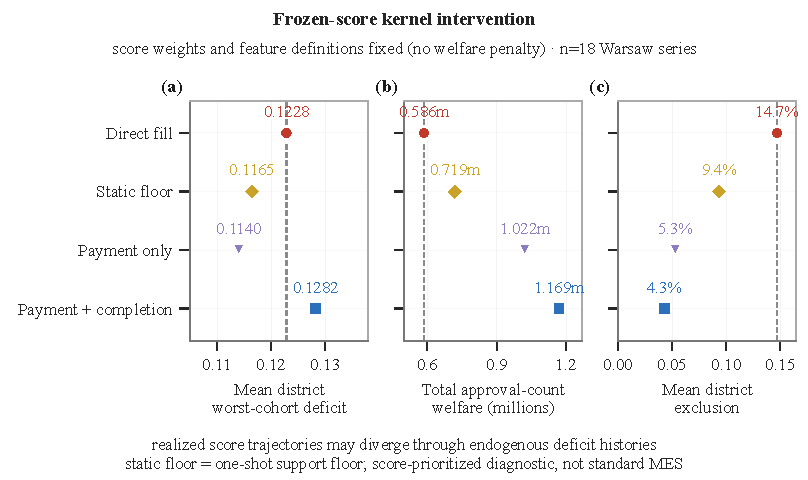
\includegraphics[width=0.98\textwidth]{fig_hack.pdf}
\caption{Frozen-score allocation-kernel intervention on
$n=\EvalSeriesN{}$ Warsaw district series. The panels compare mean worst-group
CSD, total approval-count welfare, and mean exclusion under
direct fill, a one-shot support floor, score-prioritized approver-funded
payment, and payment plus completion. Score weights and feature definitions
remain fixed. Realized score trajectories may still diverge because each rule
generates its own deficit history. Payment plus completion lowers exclusion
from \KernelDirectExcl{} to \KernelPaymentCompleteExcl{} and multiplies welfare
by \KernelPaymentCompleteWelfareFactor$\times$; the CSD change is not detectable
($p$~\KernelPaymentCompleteCSDP). The diagnostic is not standard \MES{} and
provides neither a universal nor an external guarantee.}
\label{fig:hack}
\end{figure}

The following tables use the same result files as the main text. They report
the values for each series, seed, partition, and condition that underlie the
aggregates.

\begin{table}[tb]
\centering\small
\begin{tabular}{lccc}
\toprule
Condition (no welfare penalty) & Mean worst-group $\csd$ & Welfare & Exclusion \\
\midrule
Outcome family, unconstrained & \LearnedCornerCSD & \LearnedCornerWelfare & \LearnedCornerExcl \\
\quad + support floor $\kappa = 1$ & \IdentKOneCSD & \IdentKOneWelfare & \IdentKOneExcl \\
\quad + support floor $\kappa = 2$ & \IdentKTwoCSD & \IdentKTwoWelfare & \IdentKTwoExcl \\
\midrule
Learned endowment map (reference) & \EndowCSD & \EndowWelfare & \EndowExcl \\
\MES{} (reference) & \TestMESCSD & \TestMESWelfare & \TestMESExcl \\
\bottomrule
\end{tabular}
\caption{Retrained static-floor control for Proposition~\ref{prop:support}. We
fit the outcome family with \emph{no welfare penalty}. The support floor adds
a one-shot coverage restriction without iterative approver payment.
At $\kappa=1$, all three reported outcomes improve over the unconstrained
policy, yet welfare remains roughly forty percent below Equal Shares and
exclusion roughly twice as high. Table~\ref{tab:kernel-intervention} instead
holds the learned score weights fixed and introduces payment dynamics
separately.}
\label{tab:identification}
\end{table}

\label{app:tables}

\begin{table}[t]
\centering\small
\begin{tabular}{lccccc}
\toprule
& Welfare target $\tau$ & Worst $\csd$ & Mean $\csd$ & Welfare & Exclusion \\
\midrule
\multicolumn{6}{l}{\emph{Endowment family (mechanism retained)}}\\
& 0.00 & 0.1743 & 0.0374 & 1,274,522 & 0.0418 \\
& 0.99 & 0.1736 & 0.0371 & 1,277,125 & 0.0418 \\
& 1.00 & 0.1876 & 0.0395 & 1,284,042 & 0.0433 \\
\midrule
\multicolumn{6}{l}{\emph{Outcome family (mechanism discarded)}}\\
& 0.00 & 0.1228 & 0.0024 & 586,114 & 0.1470 \\
& 0.85 & 0.1153 & 0.0101 & 1,198,311 & 0.0450 \\
& 0.95 & 0.1483 & 0.0228 & 1,259,890 & 0.0442 \\
& 1.00 & 0.1728 & 0.0320 & 1,303,057 & 0.0447 \\
& 1.02 & 0.1828 & 0.0352 & 1,310,536 & 0.0451 \\
& 1.05 & 0.1869 & 0.0364 & 1,312,691 & 0.0450 \\
\bottomrule
\end{tabular}
\caption{Sweeps over soft welfare targets for both arms at seed 42 on held-out Warsaw districts. Worst $\csd$ is the equal-weight mean district-level worst-group value; lower CSD and exclusion and higher welfare are favorable. Targets are penalties, not hard constraints. This single-seed descriptive sweep has no intervals; corpus- and budget-specific ranges are not universal reachable sets.}
\label{tab:endowfrontier}
\end{table}



\section{Additional robustness and diagnostic tables}
\label{sec:scheme}

\paragraph{Group-partition robustness.}
The main analysis partitions voters by age~$\times$~sex, and the objective is
defined relative to that choice. We therefore rescore the same fitted policies
under coarser partitions. The policies remain those trained on the original
groups. No model is refitted.



Both learned policies remain ahead of Equal Shares for every tested partition
($p \le \PartMaxLearnedP$ in exact paired sign-flip tests). These dependent
rescores evaluate the same allocations and provide no independent transfer
evidence. Absolute deficits fall for coarser groups because averaging over
fewer, larger groups removes variation, but the policy differences remain.

Greedy approvals per cost changes rank across partitions: it beats Equal Shares
under \texttt{age} and loses under \texttt{sex}. Rollover Equal Shares has
slightly lower mean CSD than Equal Shares under both coarser partitions:
\PartAgeRESCSD{} versus \PartAgeMESCSD{} for age and
\PartSexRESCSD{} versus \PartSexMESCSD{} for sex.

\clearpage
\paragraph{Support-floor separator.}\mbox{}\par

\begin{table}[H]
\centering
\small
\begin{tabular}{lcc}
\toprule
Policy & \% of funded projects & \% of budget \\
\midrule
Greedy (approvals/cost) & \InfeasGreedyCostProj & \InfeasGreedyCostBudget \\
\MES{} & \InfeasMESProj & \InfeasMESBudget \\
Learned endowment map & \InfeasLearnedEndowProj & \InfeasLearnedEndowBudget \\
Learned outcome (soft target $1.0$) & \InfeasOutcomeHeadProj & \InfeasOutcomeHeadBudget \\
\midrule
Learned outcome (unconstrained) & \textbf{\InfeasOutcomeCornerProj} & \textbf{\InfeasOutcomeCornerBudget} \\
\bottomrule
\end{tabular}
\caption{Spending on projects below the $\kappa=1$ payment-phase support floor,
$|A(p)|/|N| < c(p)/b$. The unpenalized direct policy spends
\InfeasOutcomeCornerBudget{} of its budget on such projects. Every tested
payment-based rule stays below one percent. For uniform Equal Shares, these
projects enter through completion. Nonuniform learned endowments need not
satisfy the $\kappa=1$ floor during payment. This comparison describes the
observed policies, not a universal feasible region.}
\label{tab:infeasible}
\end{table}

\paragraph{Outcome-feature ablation.}\mbox{}\par

\begin{table}[H]
\centering\small
\begin{tabular}{lcc}
\toprule
Feature removed & Mean worst-group $\csd$ & $\Delta$ vs full \\
\midrule
Cost share & \AblCostShareCSD & \AblCostShareDelta \\
Approvals per cost & \AblPerCostCSD & \AblPerCostDelta \\
Deficit-weighted support & \AblDeficitCSD & \AblDeficitDelta \\
Approval share & \AblApprShareCSD & \AblApprShareDelta \\
Cohort concentration & \AblConcCSD & \textbf{\AblConcDelta} \\
\bottomrule
\end{tabular}
\caption{Leave-one-feature-out results for direct scores. Each variant is
refitted once with the full model's optimization budget and evaluated on
held-out elections. Removing cohort concentration, which identifies projects
with demographically balanced support, improves held-out CSD by the largest
amount in this single-refit comparison.}
\label{tab:ablation}
\end{table}

\paragraph{Remaining generated tables.}
The appendix tables read the same stored result files and generated values as
the main text. Table~\ref{tab:kernel-intervention} reports the frozen-score
replay at three soft targets, and Table~\ref{tab:perseries} lists every series
at the headline operating point, including the losses. Tables
\ref{tab:district-cv} and~\ref{tab:district-bound} give the disjoint-series
contrasts and post hoc coefficient-box sensitivity. Table~\ref{tab:seeds}
reports seed sensitivity, while Table~\ref{tab:twoarm} gives both learned
classes for every held-out district. Table~\ref{tab:crosscity} reports the
native-approval difference \CrossCityAllDiff{} across \CrossCitySeriesN{}
series and the actuation grid. Table~\ref{tab:schemefull} contains the complete
group-partition robustness sweep.

% AUTO-GENERATED by tempopb/src/gen_iclr_appendix.py -- do not hand-edit.
% Regenerate after any change to the underlying results CSVs.

\begin{table}[H]\centering\scriptsize
\begin{tabular}{llrrrrr}
\toprule
Soft target & Allocation kernel & Worst $\csd$ & $\Delta$ direct & Welfare & W/direct & Exclusion \\
\midrule
0.00 & direct greedy fill & 0.1228 & +0.0000 & 586,114 & 1.00 & 0.1470 \\
 & direct + static floor ($\kappa=1$) & 0.1165 & -0.0064 & 719,168 & 1.23 & 0.0935 \\
 & iterative payment only & 0.1140 & -0.0088 & 1,021,566 & 1.74 & 0.0530 \\
 & iterative payment + completion & 0.1282 & +0.0054 & 1,168,671 & 1.99 & 0.0427 \\
0.85 & direct greedy fill & 0.1153 & +0.0000 & 1,198,311 & 1.00 & 0.0450 \\
 & direct + static floor ($\kappa=1$) & 0.1340 & +0.0187 & 1,218,887 & 1.02 & 0.0434 \\
 & iterative payment only & 0.1605 & +0.0452 & 1,132,666 & 0.95 & 0.0534 \\
 & iterative payment + completion & 0.1836 & +0.0683 & 1,273,668 & 1.06 & 0.0430 \\
1.00 & direct greedy fill & 0.1728 & +0.0000 & 1,303,057 & 1.00 & 0.0447 \\
 & direct + static floor ($\kappa=1$) & 0.1799 & +0.0071 & 1,302,820 & 1.00 & 0.0449 \\
 & iterative payment only & 0.1786 & +0.0058 & 1,130,853 & 0.87 & 0.0570 \\
 & iterative payment + completion & 0.1979 & +0.0251 & 1,289,024 & 0.99 & 0.0431 \\
\bottomrule\end{tabular}
\caption{Allocation-kernel replay over held-out Warsaw district series. Within each target, $\Delta$ is kernel minus direct-greedy CSD; negative values favor the kernel, as do lower exclusion and higher welfare. Values are descriptive without intervals. Score weights and feature definitions are fixed, but history-dependent values and scores may diverge. The static floor uses Proposition~\ref{prop:support} at $\kappa=1$; uniform-balance score-prioritized payment is diagnostic, not standard \MES{}.}
\label{tab:kernel-intervention}\end{table}

\begin{table}[t]\centering\scriptsize
\begin{tabular}{llrrrrr}
\toprule
Seed & City & $\Delta$ CSD $\downarrow$ & 95\% paired-bootstrap interval & Holm $p$ & $\Delta$ exclusion $\downarrow$ & Welfare ratio $\uparrow$ \\
\midrule
1 & Katowice & -0.0125 & [-0.0307, 0.0016] & -- & +0.0078 & 0.9913 \\
1 & Krakow & -0.0138 & [-0.0407, 0.0082] & -- & +0.0037 & 1.0014 \\
2 & Katowice & -0.0027 & [-0.0080, 0.0000] & -- & +0.0010 & 1.0002 \\
2 & Krakow & -0.0080 & [-0.0278, 0.0051] & -- & -0.0014 & 1.0015 \\
42 & Katowice & -0.0117 & [-0.0282, 0.0000] & 0.5000 & +0.0085 & 0.9924 \\
42 & Krakow & -0.0026 & [-0.0259, 0.0166] & 0.8398 & +0.0015 & 1.0041 \\
\bottomrule\end{tabular}
\caption{Projected-support-set results by city and frozen seed, with series as paired analysis units. $\Delta$ is learned endowment minus Equal Shares, so negative values favor the learned map. Intervals use paired-series bootstrap resampling, and Holm-adjusted $p$ values are shown only for the primary seed. Ballot projection limits the transfer interpretation.}
\label{tab:external-city-seed}\end{table}

\begin{table}[t]\centering\scriptsize
\begin{tabular}{lrl}
\toprule
Frozen condition & Observed & Status \\
\midrule
city macro $\leq -0.005$ for every seed & maximum -0.0054 & \checkmark \\ 
negative in each city for every seed & 6/6 negative & \checkmark \\ 
primary paired-bootstrap interval excludes zero in each city & Katowice 0.0000, Krakow 0.0166 & \texttimes \\ 
primary Holm $p \leq 0.05$ in each city & Katowice 0.5000, Krakow 0.8398 & \texttimes \\ 
welfare ratio $\geq 0.98$ in each city and seed & minimum 0.9913 & \checkmark \\ 
exclusion increase $\leq 0.005$ in each city and seed & maximum 0.0085 & \texttimes \\ 
endowment actuation $\geq 8$ and greater than priority & 12 versus 3 series & \checkmark \\ 
city-macro seed spread $\leq 0.005$ & 0.0078 & \texttimes \\ 
\bottomrule\end{tabular}
\caption{One row per preregistered condition for the projected-support-set external study, judged in the direction printed in the condition. The deterministic joint status is \texttt{falsified} because the verdict is conjunctive and not all conditions pass.}
\label{tab:external-gates}\end{table}

\begin{table}[t]\centering\scriptsize
\begin{tabular}{lllll}
\toprule
Version & Lock SHA-256 prefix & Stage & Metrics computed & Classification \\
\midrule
\texttt{v1} & \texttt{064957412947} & approval-only abort & No---no scientific result & protocol\_invalid \\
\texttt{v2} & \texttt{1464a34e2274} & Unicode-label technical abort & No---no scientific result & technical\_invalid \\
\texttt{v3} & \texttt{a6d7f945b6f6} & valid amended run & Yes & falsified \\
\bottomrule\end{tabular}
\caption{v1 and v2 ended before metrics were computed. Only v3 contributes results. Matching hashes authenticate the artifacts, not the transfer claim.}
\label{tab:external-lineage}\end{table}

\begin{table}[t]\centering\small
\begin{tabular}{lccccc}
\toprule
Series & Test years & \MES{} & Learned outcome & $\Delta$ & Worst group \\
\midrule
Wesoła & 2023, 2024, 2025 & 0.2727 & 0.1359 & -0.1368 & 60+ (M) \\
Praga-Północ & 2023, 2024, 2025 & 0.1953 & 0.1119 & -0.0833 & 60+ (M) \\
Praga-Południe & 2023, 2024, 2025 & 0.2333 & 0.1808 & -0.0524 & 60+ (M) \\
Włochy & 2023, 2024, 2025 & 0.1178 & 0.0696 & -0.0482 & 25-39 (M) \\
Wola & 2023, 2024, 2025 & 0.1933 & 0.1501 & -0.0432 & 60+ (M) \\
Rembertów & 2023, 2024, 2025 & 0.1665 & 0.1264 & -0.0401 & 60+ (M) \\
Bemowo & 2023, 2024, 2025 & 0.1583 & 0.1185 & -0.0397 & 60+ (M) \\
Bielany & 2023, 2024, 2025 & 0.1056 & 0.0693 & -0.0363 & 40-59 (M) \\
Ursus & 2023, 2024, 2025 & 0.2338 & 0.2010 & -0.0328 & 60+ (F) \\
Mokotów & 2023, 2024, 2025 & 0.2917 & 0.2691 & -0.0226 & 60+ (M) \\
Ursynów & 2023, 2024, 2025 & 0.0802 & 0.0684 & -0.0118 & 40-59 (M) \\
Wawer & 2023, 2024, 2025 & 0.1580 & 0.1517 & -0.0062 & 60+ (M) \\
Śródmieście & 2023, 2024, 2025 & 0.2624 & 0.2578 & -0.0046 & 60+ (M) \\
Targówek & 2023, 2024, 2025 & 0.1697 & 0.1676 & -0.0021 & 60+ (M) \\
Ochota & 2023, 2024, 2025 & 0.2091 & 0.2131 & \textbf{+0.0040} & 60+ (M) \\
Żoliborz & 2023, 2024, 2025 & 0.3083 & 0.3153 & \textbf{+0.0070} & <25 (M) \\
Wilanów & 2023, 2024, 2025 & 0.2552 & 0.2656 & \textbf{+0.0104} & 60+ (M) \\
Białołęka & 2023, 2024, 2025 & 0.1737 & 0.2383 & \textbf{+0.0645} & 60+ (M) \\
\bottomrule\end{tabular}
\caption{Per-series worst-group CSD for the learned outcome policy at soft target 1.00 on held-out Warsaw editions. $\Delta$ is learned minus Equal Shares; negative values favor learned and positive losses are bold. Rows are descriptive without intervals. The aggregate is the equal-weight mean district-level worst-group CSD, all from one city.}
\label{tab:perseries}\end{table}

\begin{table}[t]\centering\small
\begin{tabular}{lrrr}
\toprule
Rollover intensity $\lambda$ & Worst $\csd$ & Welfare & Exclusion \\
\midrule
0.00 & 0.1992 & 1,293,610 & 0.0438 \\
0.25 & 0.1977 & 1,292,741 & 0.0435 \\
0.50 & 0.1983 & 1,288,507 & 0.0433 \\
0.75 & 0.1987 & 1,287,880 & 0.0436 \\
1.00 & 0.1951 & 1,286,793 & 0.0436 \\
\bottomrule\end{tabular}
\caption{All tested rollover intensities on held-out Warsaw editions. Lower CSD and exclusion and higher welfare are favorable; the former are equal-weight district-series means and welfare is summed. Rows are descriptive without intervals. $\lambda=0$ is Equal Shares; $\lambda=1$ is the main-text reference and optimizer initial mean, not selected on held-out results.}
\label{tab:res-grid}\end{table}

\begin{table}[t]\centering\small
\begin{tabular}{lccccc}
\toprule
Soft welfare target & seed 1 & seed 2 & seed 3 & seed 42 & spread \\
\midrule
0.00 & 0.1123 & 0.1217 & 0.1089 & 0.1228 & 0.0139 \\
0.85 & 0.1126 & 0.1150 & 0.1277 & 0.1153 & 0.0151 \\
0.95 & 0.1295 & 0.1489 & 0.1171 & 0.1483 & 0.0318 \\
1.00 & 0.1695 & 0.1735 & 0.1702 & 0.1728 & 0.0040 \\
1.02 & 0.1823 & 0.1842 & 0.1795 & 0.1828 & 0.0047 \\
1.05 & 0.1821 & 0.1879 & 0.1821 & 0.1869 & 0.0058 \\
\bottomrule\end{tabular}
\caption{Outcome-frontier seed sensitivity on held-out Warsaw district series. Cells are equal-weight mean district-level worst-group CSD (lower is favorable); spread is the fitted-seed range and describes optimization sensitivity, not sampling uncertainty.}
\label{tab:seeds}\end{table}

\begin{table}[t]\centering\small
\begin{tabular}{llccccc}
\toprule
Partition & Policy & Worst $\csd$ & vs \MES{} & $p$ & Wins \\
\midrule
age $\times$ sex (8) & mes & 0.1992 & -- & -- & -- \\
 & res-1.0 & 0.1951 & -- & -- & -- \\
 & greedy-cost & 0.1991 & -- & -- & -- \\
 & learned-endowment & 0.1736 & -0.0255 & 0.0115 & 11/18 \\
 & learned-outcome & 0.1728 & -0.0264 & 0.0130 & 14/18 \\
age (4) & mes & 0.1127 & -- & -- & -- \\
 & res-1.0 & 0.1106 & -- & -- & -- \\
 & greedy-cost & 0.1081 & -- & -- & -- \\
 & learned-endowment & 0.0907 & -0.0220 & 0.0079 & 14/18 \\
 & learned-outcome & 0.0815 & -0.0312 & 0.0093 & 13/18 \\
sex (2) & mes & 0.0585 & -- & -- & -- \\
 & res-1.0 & 0.0558 & -- & -- & -- \\
 & greedy-cost & 0.0759 & -- & -- & -- \\
 & learned-endowment & 0.0352 & -0.0233 & $<0.001$ & 14/18 \\
 & learned-outcome & 0.0224 & -0.0361 & $<0.001$ & 17/18 \\
\bottomrule\end{tabular}
\caption{Held-out Warsaw district series rescored under each group partition. ``vs \MES{}'' is policy minus Equal Shares; negative values, paired exact sign-flip $p$ values, and wins use series. Age~$\times$~sex policies are rescored without refitting, so rows are dependent robustness checks, not transfer evidence.}
\label{tab:schemefull}\end{table}

\begin{table}[t]\centering\scriptsize
\begin{tabular}{lrrrrrrr}
\toprule
Baseline & Learned $\csd$ & Base $\csd$ & $\Delta$ & 95\% $\Delta$ interval & $p_{\rm fold}$ & Series wins & Fold wins \\
\midrule
greedy-cost & 0.1941 & 0.2161 & -0.0220 & [-0.0385, -0.0056] & 0.0625 & 13/19 & 5/5 \\
greedy-count & 0.1941 & 0.2466 & -0.0525 & [-0.0703, -0.0364] & 0.0625 & 19/19 & 5/5 \\
LLMRule count & 0.1941 & 0.2294 & -0.0353 & [-0.0495, -0.0223] & 0.0625 & 17/19 & 5/5 \\
LLMRule cost & 0.1941 & 0.2375 & -0.0434 & [-0.0593, -0.0293] & 0.0625 & 18/19 & 5/5 \\
\MES{} & 0.1941 & 0.2242 & -0.0301 & [-0.0396, -0.0205] & 0.0625 & 17/19 & 5/5 \\
\RES{} $(\lambda=1)$ & 0.1941 & 0.2225 & -0.0284 & [-0.0376, -0.0194] & 0.0625 & 18/19 & 5/5 \\
\bottomrule\end{tabular}
\caption{Five-fold out-of-district contrasts over 19 series, each scored by a map fitted on the other districts. This is not a temporal holdout and not cross-city validation: 18 of the 19 series are Warsaw districts. $\Delta$ is learned minus baseline; negative values favor learned. Paired-series bootstrap intervals are descriptive over 19 series. $p_{\rm fold}$ is an exact sign-flip dependence sensitivity check on fold means (minimum two-sided resolution 0.0625). Overlapping training sets make folds dependent.}
\label{tab:district-cv}\end{table}

\begin{table}[t]\centering\scriptsize
\begin{tabular}{@{}lrrrrrrrrr@{}}
\toprule
Weight box & Learned & \MES{} & $\Delta$ & 95\% $\Delta$ interval & $p_{\rm fold}$ & S-win & F-win & W/\MES{} & Excl. \\
\midrule
10 (primary) & 0.1941 & 0.2242 & -0.0301 & [-0.0396, -0.0205] & 0.0625 & 17/19 & 5/5 & 0.984 & 0.0628 \\
40 (post hoc) & 0.1886 & 0.2242 & -0.0355 & [-0.0477, -0.0235] & 0.0625 & 17/19 & 5/5 & 0.983 & 0.0645 \\
\bottomrule\end{tabular}
\caption{Post hoc fourfold box-expansion sensitivity on held-out series. Bound-10 is the primary analysis; bound 40 is post hoc. $\Delta$ is learned minus Equal Shares; negative favors learned. Intervals use paired series; $p_{\rm fold}$ tests fold-mean signs under dependence. S-win and F-win count series and fold-mean wins. This is an outcome stability check, not coefficient identification or independent replication.}
\label{tab:district-bound}\end{table}

\begin{table}[t]\centering\scriptsize
\begin{tabular}{lrrrrlr}
\toprule
Scope & Learned $\csd$ & \MES{} $\csd$ & $\Delta$ & 95\% $\Delta$ interval & $p$ & Wins \\
\midrule
Gdynia & 0.1301 & 0.1375 & -0.0074 & [-0.0197, +0.0000] & 0.500 & 2/22 \\
\L{}\'od\'z & 0.1373 & 0.1390 & -0.0017 & [-0.0120, +0.0077] & 0.736 & 10/36 \\
Both cities & 0.1345 & 0.1384 & -0.0039 & [-0.0114, +0.0031] & 0.316 & 12/58 \\
\midrule
\multicolumn{7}{l}{\emph{Actuation by instance granularity (whole prespecified grid)}} \\
Min.\ projects/election & Series & Inert & $\Delta$ & 95\% $\Delta$ interval & $p$ & Wins/losses \\
\midrule
$\ge$ 0 & 58 & 36 & -0.0039 & [-0.0114, +0.0031] & 0.316 & 12/10 \\
$\ge$ 5 & 43 & 21 & -0.0052 & [-0.0155, +0.0040] & 0.315 & 12/10 \\
$\ge$ 10 & 29 & 10 & -0.0026 & [-0.0155, +0.0089] & 0.682 & 10/9 \\
$\ge$ 15 & 20 & 5 & -0.0022 & [-0.0102, +0.0056] & 0.605 & 7/8 \\
$\ge$ 20 & 17 & 4 & -0.0024 & [-0.0118, +0.0069] & 0.640 & 6/7 \\
$\ge$ 25 & 10 & 1 & -0.0007 & [-0.0117, +0.0101] & 0.969 & 4/5 \\
$\ge$ 30 & 5 & 0 & +0.0015 & [-0.0151, +0.0205] & 0.938 & 3/2 \\
\bottomrule\end{tabular}
\caption{Native-approval Gdynia and \L{}\'od\'z series scored from 2023 with the frozen Warsaw map, without refitting or support-set projection. $\Delta$ is learned minus Equal Shares; negative favors learned. Paired-series bootstrap intervals summarize uncertainty. \emph{Inert} means the Equal Shares allocation (median projects: 6.2 inert, 22.2 active). Effects stay near zero across the prespecified grid, so low actuation alone does not explain the null. $p$ uses exact sign flips when feasible and 200{,}000 draws otherwise. Two cities do not establish wider validity.}
\label{tab:crosscity}\end{table}

\begin{table}[t]\centering\scriptsize
\begin{tabular}{lrrrrr}
\toprule
Series & \MES{} & Endowment & $\Delta$ & Direct & $\Delta$ \\
\midrule
Żoliborz & 0.3083 & 0.1726 & -0.1357 & 0.3153 & \textbf{+0.0070} \\
Praga-Północ & 0.1953 & 0.1093 & -0.0860 & 0.1119 & -0.0833 \\
Wesoła & 0.2727 & 0.2080 & -0.0647 & 0.1359 & -0.1368 \\
Praga-Południe & 0.2333 & 0.1773 & -0.0560 & 0.1808 & -0.0524 \\
Wawer & 0.1580 & 0.1080 & -0.0500 & 0.1517 & -0.0062 \\
Ursynów & 0.0802 & 0.0461 & -0.0342 & 0.0684 & -0.0118 \\
Ursus & 0.2338 & 0.2062 & -0.0276 & 0.2010 & -0.0328 \\
Włochy & 0.1178 & 0.0942 & -0.0236 & 0.0696 & -0.0482 \\
Mokotów & 0.2917 & 0.2733 & -0.0184 & 0.2691 & -0.0226 \\
Wilanów & 0.2552 & 0.2410 & -0.0141 & 0.2656 & \textbf{+0.0104} \\
Wola & 0.1933 & 0.1813 & -0.0120 & 0.1501 & -0.0432 \\
Rembertów & 0.1665 & 0.1665 & +0.0000 & 0.1264 & -0.0401 \\
Śródmieście & 0.2624 & 0.2624 & +0.0000 & 0.2578 & -0.0046 \\
Białołęka & 0.1737 & 0.1764 & \textbf{+0.0027} & 0.2383 & \textbf{+0.0645} \\
Bemowo & 0.1583 & 0.1613 & \textbf{+0.0030} & 0.1185 & -0.0397 \\
Bielany & 0.1056 & 0.1087 & \textbf{+0.0031} & 0.0693 & -0.0363 \\
Ochota & 0.2091 & 0.2257 & \textbf{+0.0166} & 0.2131 & \textbf{+0.0040} \\
Targówek & 0.1697 & 0.2070 & \textbf{+0.0373} & 0.1676 & -0.0021 \\
\bottomrule\end{tabular}
\caption{Headline learned endowment and direct-outcome policies by held-out Warsaw district, ordered by endowment contrast. Each $\Delta$ is policy minus Equal Shares; negative favors learned and positive losses are bold. Rows are descriptive without intervals.}
\label{tab:twoarm}\end{table}


\end{document}
